\documentclass[xcolor=x11names]{beamer}
%%%%%%%%%%%%%%%%%%%%%%%%%%%%%%%%%%%%%%%%%%%%%%%%%%%%%%%%%%%%
%%  This Beamer template was created by Cameron Bracken.
%%  Anyone can freely use or modify it for any purpose
%%  without attribution.
%%
%%  Last Modified by C. Bracken: January 9, 2009
%%
%%  The preamble, and maybe some modification of the Cameron Bracken's template is due to Attila Molnár.
%%
%%

%% General document
\usepackage[utf8]{inputenc}
\usepackage[T1]{fontenc}
\usepackage{graphicx}
\usepackage{tikz}
\usetikzlibrary{decorations.fractals}
\usetikzlibrary{decorations.text}
\usepgflibrary{arrows}
\usetikzlibrary{fadings}
\usetikzlibrary[decorations.pathmorphing]
\tikzfading[name=fade inside, inner color=transparent!70, outer color=transparent!70]
\usetikzlibrary{calc}
\usetikzlibrary{intersections}
\usetikzlibrary{shapes}
\usetikzlibrary{patterns}
\usefonttheme{serif}
\usepackage{amssymb} 			
\usepackage{amsmath}
\usepackage{ifthen}
\usepackage[normalem]{ulem}
\usepackage{mathrsfs}

%%%%%%%%%%%%%%%%%%%%%%%%%%%%%%%%%%%%%%%%%%%%%%%%%%%%%%%%%%%%%%%%%%%%%%%%%%%%%%%%%%%%
%% Beamer Layout %%%%%%%%%%%%%%%%%%%%%%%%%%%%%%%%%%
\useoutertheme[subsection=false,shadow]{miniframes}
\useinnertheme{default}
\usefonttheme{serif}
%\usepackage{txfonts} %Hook for strict implication!
\DeclareSymbolFont{symbolsC}{U}{txsyc}{m}{n}
\DeclareMathSymbol{\strictif}{\mathrel}{symbolsC}{74}
\DeclareMathSymbol{\boxright}{\mathrel}{symbolsC}{128}
\usepackage{palatino}
%\usepackage[uppercase=upright,charter]{mathdesign}

\setbeamerfont{title like}{shape=\scshape}
\setbeamerfont{frametitle}{shape=\scshape}


\setbeamercolor*{lower separation line head}{bg=white!40!DeepSkyBlue3}
\setbeamercolor*{normal text}{fg=black,bg=white}
\setbeamercolor*{alerted text}{fg=red}
\setbeamercolor*{example text}{fg=black}
\setbeamercolor*{structure}{fg=black}

\setbeamercolor*{palette tertiary}{fg=black,bg=white!90!DeepSkyBlue3}
\setbeamercolor*{palette quaternary}{fg=black,bg=black!10}

%\setbeamercolor{block body alerted}{bg=normal text.bg!90!DeepSkyBlue4}
\setbeamercolor{block body}{bg=normal text.bg!95!DeepSkyBlue3}
%\setbeamercolor{block body example}{bg=normal text.bg!90!DeepSkyBlue4}
%\setbeamercolor{block title alerted}{use={normal text,alerted text},fg=alerted text.fg!75!normal text.fg,bg=normal text.bg!90!DeepSkyBlue4}
\setbeamercolor{block title}{bg=normal text.bg!70!DeepSkyBlue3}
%\setbeamercolor{block title example}{use={normal text,example text},fg=example text.fg!75!normal text.fg,bg=normal text.bg!75!DeepSkyBlue4}

\setbeamertemplate{blocks}[rounded][shadow=true]
%\setbeamertemplate{background canvas}[vertical shading][bottom=white,top=structure.fg!25]
%\setbeamertemplate{sidebar canvas left}[horizontal shading][left=white!40!black,right=black]
\setbeamertemplate{itemize items}[circle]
\setbeamercolor*{itemize item}{fg=DeepSkyBlue3}
\setbeamercolor*{itemize subitem}{fg=DeepSkyBlue3}
\setbeamercolor*{itemize subsubitem}{fg=DeepSkyBlue3}
\setbeamertemplate{enumerate items}[circle]
%\setbeamercolor{item projected}{bg=DeepSkyBlue3,fg=black}
\setbeamercolor{item projected}{bg=white,fg=DeepSkyBlue3}
\setbeamercolor*{enumerate item}{fg=DeepSkyBlue3}
\setbeamercolor*{enumerate subitem}{fg=DeepSkyBlue3}
\setbeamercolor*{enumerate subsubitem}{fg=DeepSkyBlue3}

%%%%%%%%%%%%%%%%%%%%%%%%%%%%%%%%%%%%%%%%%%%%%%%%%%


%%%%%%%%%%%%%%%%%%%%%%%%%%%%%%%%%%%%%%%%%%%%%%%%%%%%%%%%%%%%%%%%%%%%%%%%%%%%%%%%%%%%

\newenvironment{defi}[1][]{\begin{block}{\footnotesize \textsc{Definition} \ifthenelse{\equal{#1}{}}{}{\, (#1)}}}{\end{block}}
\newenvironment{prop}[1][]{\begin{block}{\footnotesize \textsc{Proposition} \ifthenelse{\equal{#1}{}}{}{\, (\textsc{#1})}}}{\end{block}}
\newenvironment{lemm}[1][]{\begin{block}{\footnotesize \textsc{Lemma} \ifthenelse{\equal{#1}{}}{}{\, (\textsc{#1})}}}{\end{block}}
\newenvironment{idea}[1][]{\begin{block}{\footnotesize \textsc{Idea} \ifthenelse{\equal{#1}{}}{}{\, (\textsc{#1})}}}{\end{block}}
\newenvironment{rema}[1][]{\begin{block}{\footnotesize \textsc{Remark} \ifthenelse{\equal{#1}{}}{}{\, (\textsc{#1})}}}{\end{block}}
\newenvironment{coro}[1][]{\begin{block}{\footnotesize \textsc{Corollary} \ifthenelse{\equal{#1}{}}{}{\, (\textsc{#1})}}}{\end{block}}
\newenvironment{tete}[1][]{\begin{block}{\footnotesize \textsc{Theorem} \ifthenelse{\equal{#1}{}}{}{\, (\textsc{#1})}}}{\end{block}}
\newenvironment{claim}[1][]{\begin{block}{Claim \ifthenelse{\equal{#1}{}}{}{\, (\textsc{#1})}}}{\end{block}}
%\newenvironment{lemma}[1][]{\begin{block}{Lemma \ifthenelse{\equal{#1}{}}{}{\, (\textsc{#1})}}}{\end{block}}
\newenvironment{question}[1][]{\begin{block}{Question \ifthenelse{\equal{#1}{}}{}{\, (\textsc{#1})}}}{\end{block}}
\newenvironment{rem}[1][]{\begin{block}{Remark \ifthenelse{\equal{#1}{}}{}{\, (\textsc{#1})}}}{\end{block}}
\newenvironment{homework}[1][]{\begin{block}{Homework \ifthenelse{\equal{#1}{}}{}{\, (\textsc{#1})}}}{\end{block}}
\newenvironment{proo}[1][]{\begin{block}{\footnotesize \textsc{Proof} \ifthenelse{\equal{#1}{}}{}{\, (\textsc{#1})}}}{\end{block}}

%%%%%%%%%%%%%%%%%%%%%
%% To evade unnecessary circles, mainly for \cimdia
%%%%%%%%%%%%%%%%%%%%%

\makeatletter
\let\beamer@writeslidentry@miniframeson=\beamer@writeslidentry
\def\beamer@writeslidentry@miniframesoff{%
  \expandafter\beamer@ifempty\expandafter{\beamer@framestartpage}{}% does not happen normally
  {%else
    % removed \addtocontents commands
    \clearpage\beamer@notesactions%
  }
}
\newcommand*{\miniframeson}{\let\beamer@writeslidentry=\beamer@writeslidentry@miniframeson}
\newcommand*{\miniframesoff}{\let\beamer@writeslidentry=\beamer@writeslidentry@miniframesoff}
\makeatother

%%%%%%%%%%%%%%%%%%%%%%%%%%%%%
%%%%%%%%%%%%% END %%%%%%%%%%%
%%%%%%%%%%%%%%%%%%%%%%%%%%%%%


%%%% Formatting Commands

\newcommand{\cimdia}[1] {\miniframesoff \begin{frame}\begin{center}\huge \begin{tabular}{c}#1\end{tabular}\end{center}\end{frame}\miniframeson}
\newcommand{\szakasz}[2][]{\section{#1}\subsection{}\cimdia{#2}}
\newcommand{\bluebullet}{\textcolor{DeepSkyBlue3}{\quad $\bullet$} \,\,}

\newenvironment{frame*}[1][]{\miniframesoff \begin{frame} #1}{\end{frame}\miniframeson}

  % for admissible intersections
  \newcommand{\bigsqcap}{\rotatebox[origin=c]{180}{$\bigsqcup$}}

  % Intelligent curves for tikz:
  % Use it in this way: \gorbe{elejenev}{vegenev}{elejeszog}{elejelendulet}{vegeszog}{vegelendulet};
  \newcommand{\gorbe}[6]{\draw (#1).. controls ([shift=(#3: #4 cm)]#1) and ([shift=(#5: #6 cm)]#2) .. (#2);}
  \newcommand{\gorbefelirattal}[8]{\draw (#1).. controls ([shift=(#3: #4 cm)]#1) and ([shift=(#5: #6 cm)]#2) .. (#2) node[#8] {#7};}

\newcommand{\pipa}{%
\begin{tikzpicture}[green!50!black, thick, scale=.1]
\gorbe{0,1}{2,2}{-80}{1}{225}{.7}
\end{tikzpicture}}

\newcommand{\ellentmondas}
		{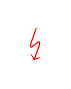
\begin{tikzpicture}[scale=0.2]
			\draw[rounded corners=3pt, rotate=10, red,
					->] (0.75,2)--(0,0.66)--(1,1.33)--(0.25,0);
		\end{tikzpicture}}
\newcommand{\indirektfelteves}
		{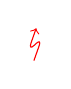
\begin{tikzpicture}[scale=0.2]
			\draw[rounded corners=3pt, rotate=10, red,
					<-] (0.75,2)--(0,0.66)--(1,1.33)--(0.25,0);
		\end{tikzpicture}}

\newcommand{\pecset}[2]{\begin{tikzpicture}[remember picture,overlay]
\node [ draw=red,
        rectangle,
        rounded corners=5mm,
        inner sep=1mm,
        ultra thick,
        fill=white,
        fill opacity=.8,
        rotate=30,
        scale=#1,
        text opacity=0.7]
        at (current page.center)
        {#2};
\end{tikzpicture}}

%\felirat{inner sep}{rounded corners}{scale}{x}{y}{text}
\newcommand{\felirat}[6]{\begin{tikzpicture}[remember picture,overlay]
\node [ draw=DeepSkyBlue3,
        rectangle,
        rounded corners=#2 mm,
        inner sep=#1mm,
        ultra thick,
        fill=white,
        fill opacity=.8,
        rotate=0,
        scale=#3,
        text opacity=1]
        at ([xshift=#4 cm, yshift=#5 cm]current page.center)
        {#6};
\end{tikzpicture}}


% Emphasizing:
\definecolor{barna}{rgb}{0.5,0.2,0.1}
\newcommand{\bemph}[1] {{\color{DeepSkyBlue3}{#1}}}
\newcommand{\kemph}[1] {{\color{blue}{#1}}}
\newcommand{\cemph}[1]{\textcolor{red}{#1}}
\newcommand{\zemph}[1] {{\color{Green2}{#1}}}
\newcommand{\yemph}[1] {{\color{Orange1}{#1}}}
\renewcommand{\emph}[1]{\textbf{#1}}

% i dont know whats this
\newcommand{\matbuborek}[1]{%
\begin{tikzpicture}
\node[draw=black, rounded corners=2pt, rectangle, inner sep=1mm] at (0,0){$#1$};
\end{tikzpicture}}



% modal operators:
 \newcommand{\diamondmeret}{.18}
 \newcommand{\boxmeret}{4*\diamondmeret/5}

 \newcommand{\PD}[1]{
  \mathop{\raisebox{-.5ex}{$\begin{tikzpicture}[scale=\diamondmeret]
  \draw[rounded corners=1pt, thick] (1,0)--(0,1)--(-1,0)--(0,-1)--cycle;
  \node[inner sep=0pt] at (0,0) {\tiny #1};
  \end{tikzpicture}$}}}
 \newcommand{\PB}[1]{%
  \mathop{\raisebox{-.2ex}{\begin{tikzpicture}[scale=\boxmeret]
  \draw[rounded corners=1pt, thick] (-1,-1)--(1,-1)--(1,1)--(-1,1)--cycle;
  \node[inner sep=0pt] at (0,0) {\tiny #1};
  \end{tikzpicture}}}}

\newcommand{\DiamondBox}[1][]{%
\begin{tikzpicture}[baseline={([yshift=-.5ex]current bounding box.center)}]
\draw[thick, rounded corners=.3pt]
 (-.11,0) --(0,-.11) -- (.11,-.11) -- (.11,.11)-- (0,.11)--cycle;%
\node[scale=.4, inner sep=0mm] at (0.03,0){#1};
\end{tikzpicture}\hspace{1pt}}

\newcommand{\BoxDiamond}[1][]{%
\begin{tikzpicture}[scale=1,baseline={([yshift=-.5ex]current bounding box.center)}]
\draw[thick, rounded corners=.3pt]
 (-.11,-.11) -- (0,-.11) --(.11,0) -- (0,.11)-- (-.11,.11)--cycle;%
\node[inner sep=0mm] at (0,0){\footnotesize #1};
\end{tikzpicture}\hspace{1pt}}

\newcommand{\Boxi}[1][]{\Box_{#1}}
\newcommand{\BBox}[1][]{\mathop{\raisebox{.3ex}{\scalebox{.6}{$\Box$}} \hspace{-1.325ex}\Box_{#1} \hspace{-.25ex}}}
\newcommand{\BBoxDot}[1][]{\mathop{\raisebox{.2ex}{$\cdot$} \hspace{-1.175ex} \BBox[#1]}}

\renewcommand{\Diamond}{\scalebox{.9}{\raisebox{-.4ex}{\rotatebox{45}{$\Box$}}}}
\newcommand{\DDiamond}{\mathop{\scalebox{.9}{\raisebox{-.4ex}{\rotatebox{45}{$\Box \hspace{-1.325ex}\raisebox{.3ex}{\scalebox{.6}{$\Box$}}$}}}}}
\newcommand{\DDiamondDot}{\mathop{\DDiamond \hspace{-1.45ex} \raisebox{.1ex}{$\cdot$}\hspace{.45ex}}}


 \newcommand{\mland} [1][.1]{\hspace{#1cm}\textup{and}\hspace{#1cm}}
 \newcommand{\mlthen}[1][.1]{\hspace{#1cm}\Rightarrow\hspace{#1cm}}
 \newcommand{\mlnot} [1][.1]{\hspace{#1cm}\textup{not }}
 \newcommand{\mlor}  [1][.1]{\hspace{#1cm}\textup{or}\hspace{#1cm}}
 \newcommand{\mliff} [1][.1]{\hspace{#1cm}\mliff\hspace{#1cm}}
 \newcommand{\vonal} [1][.2]{\hspace{#1cm} | \hspace{#1cm}}
 \newcommand{\mlwhere} [1][.2]{\hspace{#1cm}\textup{where}\hspace{#1cm}}
 \newcommand{\lrule}[3][c]{\begin{array}{#1} #2  \\  \hline #3 \end{array}}
 \newcommand{\dlrule}[3][c]{\begin{array}{#1} #2  \\  \hline\hline #3 \end{array}}
 \newcommand{\dual}{\delta}
\newcommand{\Dajmond}{\lozenge}
\newcommand{\Boksz}{\square}
\newcommand{\felDajmond}{\blacklozenge}
\newcommand{\felBoksz}{\blacksquare}
\newcommand{\felle}	
	{\,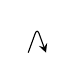
\begin{tikzpicture}
		\pgfmathsetmacro{\szog}{70}
		\pgfmathsetmacro{\hossz}{0.33}
	\draw[->,>=stealth,rounded corners=2pt] (0,0)	--(\szog:\hossz cm)
								--([shift=(-\szog :\hossz cm)]\szog:\hossz cm);	
	\end{tikzpicture}\,}
\newcommand{\lefel}
	{\, 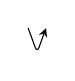
\begin{tikzpicture}
		\pgfmathsetmacro{\szog}{70}
		\pgfmathsetmacro{\hossz}{0.33}
		\draw[->,>=stealth,rounded corners=2pt] (0,0)	--(-\szog:\hossz cm)
								--([shift=(\szog :\hossz cm)]-\szog:\hossz cm);
	\end{tikzpicture}\, }
\newcommand{\enn}
{\mathbf{N}}
\newcommand{\nne}
{\reflectbox{$\mathbf{N}$}}

\newcommand{\mono}{\rightarrowtail}
\newcommand{\epi}{\twoheadrightarrow}
\newcommand{\iso}{\rightarrowtail \!\!\!\!\! \rightarrow}

 \newcommand{\defegy}[1][.1]{\hspace{#1cm}\overset{\textup{\tiny def}}{=}\hspace{#1cm}}
 \newcommand{\defpont}[1][.1]{\hspace{#1cm}\overset{\textup{\tiny def}}{:}\hspace{#1cm}}
 \newcommand{\defekv}[1][.1]{\hspace{#1cm}\overset{\textup{\tiny def}}{ \Leftrightarrow }\hspace{#1cm}}
 \newcommand{\lthen}{\rightarrow}
 \newcommand{\liff}{\leftrightarrow}
 \newcommand{\lminus}{-}
 \newcommand{\lsup}{\mbox{$\mathop{\sim}$}}
 \newcommand{\colnot}{\mbox{$\mathop{\sim}$}}
 \newcommand{\forallin}[2]{(\forall #1 \in #2)}
 \newcommand{\existsin}[2]{(\exists #1 \in #2)}
 \newcommand{\nexistsin}[2]{(\nexists #1 \in #2)}
 \newcommand{\forallp}[1]{(\forall #1)}
 \newcommand{\existsp}[1]{(\exists #1)}
 \newcommand{\forallR}[2]{(\forall #1 \reflectbox{$R$} #2)}
 \newcommand{\existsR}[2]{(\exists #1 \reflectbox{$R$} #2)}
\newcommand{\magyarazat}[2]{\overset{\substack{\textup{#2}\\ \downarrow}}{#1}}


\newcommand{\bintension}[2][]{{{[}\!{[}} {#2}{{]}\!{]}}^{\mathcal{#1}}}
\newcommand{\wintension}[3][]{{[}\hspace{-.46mm}{[} {#3}{]}\hspace{-.46mm}{]}^{\mathfrak{#1}}_{#2}}
\newcommand{\canintension}[2][]{{[}\hspace{-.46mm}{[} {#2}{]}\hspace{-.46mm}{]}_{\mathrm{#1}}}
\newcommand{\jelentes}[2]{{{[}\!{[}} {#1}{{]}\!{]}}^{{#2}}}
\newcommand{\intension}[2][]{{[}\hspace{-.46mm}{[} {#2}{]}\hspace{-.46mm}{]}^{\mathfrak{#1}}}
\newcommand{\Kintension}[2][]{|\!| {#2} |\!|^{\mathcal{#1}}}
\newcommand{\theory}[2][]{\mathrm{th}_{\mathfrak{#1}}(#2)}
\newcommand{\seenby}{\reflectbox R}
\newcommand{\derives}[1][]{\vdash_{\mathrm{#1}}}
\newcommand{\ugyanaz}[1]{\mathrel{\overset{#1}{\equiv}}}


\newcommand{\harmasosztas}[6]{

\begin{minipage}{#1\textwidth}%
#4%
\end{minipage}%
\begin{minipage}{#2\textwidth}%
#5%
\end{minipage}%
\begin{minipage}{#3\textwidth}%
#6%
\end{minipage}

}


\newcommand{\felkor}[8]{%
\begin{scope}[draw=#5,very thick,fill opacity=.15,draw opacity=.5,text opacity=1]
\draw[fill=#5]
([shift=(#3:#2)]#1) arc (#3:180+#3:#2) -- cycle;
\node at ([shift=(#7*180+#3:#2),shift=(-#7*90+135+#3:0.5*#6)]#1){#8};
\clip ([shift=(#3:#2)]#1) arc (#3:180+#3:#2);
 \draw[fill=#5] ([shift=(#7*180+#3:#2)]#1) circle (#6);
\end{scope}
}
\newcommand{\felkorvonal}[2]{
\draw[rounded corners=0] (180+#1:.25*#2 cm) arc (180+#1:360+#1:.25*#2 cm)--cycle;
}


\newcommand{\BoxTemplate}[1]{{#1} \mathop{\Box\hspace{-1.35ex} \raisebox{.5ex}{\scalebox{.5}{$\lthen$}}}}
\newcommand{\DiamondTemplate}[1]{#1\hspace{-.2ex} \mathop{\Diamond\hspace{-1.35ex} \raisebox{.4ex}{\scalebox{.5}{$\land$}}}\,}

%%%%%%%%%%%%%%%%%%%%%%%%%%%%%%%%%%%%%%%%%%%%%%%%%%%%%%
\newenvironment{tomb}[2][.1]{\arraycolsep=#1cm\begin{array}{#2}}{\end{array}}
\beamertemplatenavigationsymbolsempty


\author{Attila Moln\'ar}
\date{2014. March 21.}
\title{Axiomatization of Kripkean FOML}
\institute{ELTE}
\begin{document}


\begin{frame}
\centering
\textsc{\Large Relativistic Temporal Logic \\[1em] Introduction}

\bigskip

{ \small Attila Moln\'ar

    \textit{E\"otv\"os Lor\'and University}}

 \begin{figure}

\includegraphics[scale=.3]{elte_cimer.png}
 \end{figure}

	\today
\end{frame}

\szakasz[Intro]{Introduction}

\begin{frame}
	\frametitle{McTaggart}
\footnotesize
There are two ways about speaking about time:
\begin{itemize}
\item[A-series:] with singular predicates: ``\dots is past'', ``\dots is present'', ``\dots is future''. Note that the truth of these sentences depends on the time of the utterance. Its perspective is \emph{local}.
\item[B-series:] with ordering relations: ``\dots comes before \dots'', ``\dots comes after \dots''. The truth of these sentences does not depend on the time of the utterance. Its perspective is \emph{global}.
\end{itemize}
\end{frame}



\szakasz[Language]{Language}

\begin{frame}
	\frametitle{Language}
\footnotesize
\begin{itemize}
\item Symbols:
 \begin{itemize}
 \item Clock variables: $a, b, c,\dots $ \hfill $ClVar\defegy \{a_i \, : \, i\in \omega\}$
 \item Mathematical variables: $x, y, z, \dots$ \hfill $NVar\defegy \{x_i \, : \, i\in \omega\}$
 \item Propositional variables: $p, q, r, \dots$ \hfill $PVar\defegy \{p_i \, : \, i\in \omega\}$
 \item Mathematical constants: $\mathsf r_1, \mathsf r_2, \dots$
 \item Clock constants: $\mathsf c_1, \mathsf c_2, \dots$
 \item Mathematical function symbols: $+, \cdot$
 \item Mathematical predicate symbols: $\leq$
 \item Logical symbols: $\lnot, \land, \Diamond, =, \exists$
% \item other: $(, ), ,$
 \end{itemize}
\item Mathematical terms:
\[\tau ::=\, \,   x \vonal \mathsf r\vonal \tau_1 +\tau_2 \vonal \tau_1 \cdot \tau_2\]
\item Clock terms:
\[\tau^c ::=\, \,   a \vonal \mathsf c\]
\item Formulas:
\\
$\varphi ::=\, \,  p  \vonal \tau_1 \leq \tau_2 \vonal \tau_1 = \tau_2 \vonal \mathsf c : \tau \vonal a : \tau $
\\ \hfill $ \lnot \varphi \vonal \varphi\land \psi \vonal \Diamond \varphi \vonal \exists x \varphi\vonal \exists a \varphi $
\end{itemize}
\end{frame}

\begin{frame}[t]
\frametitle{Intended meanings:}
\footnotesize
\def\sortav{.5em}
\begin{tabular}{rl}
   $a:\tau$& Clock $a$ shows the time $\tau$.
\pause
\\[\sortav] $\Diamond \varphi$& It is visible that $\varphi$.
\\[\sortav]                    & Somewhere in the \cemph{lightlike past} it was the case that $\varphi$.
\pause
\\[\sortav] $\Box \varphi$    & Everywhere in the lightlike past it was the case that $\varphi$.
\pause
\\[\sortav] $\Diamond\Diamond \varphi $& Somewhere in the \cemph{causal past} it was the case that $\varphi$.
\pause
\\[\sortav] $\Box\Box \varphi $&  Everywhere in the causal past it was the case that $\varphi$.
\pause
\\[\sortav] $\Diamond\Diamond (a:\tau \land \varphi) $& \cemph{When the clock $a$ showed $\tau $}, it was the case that $\varphi$.
\pause
\\[\sortav] $\Diamond\Diamond (\exists x\, a:x \land \varphi) $& Somewhere in the \cemph{causal past of $a$} it was the case that $\varphi$.
\pause
\\[\sortav] $p$& $p$ happened, where $p$ is some contingent event,
\\& such as ``a coin was flipped'',
\\& ``something flashed'', ``Somebody is happy'', etc.
\end{tabular}

\end{frame}


\begin{frame}[t]
\frametitle{Notations}
\footnotesize
\def\sortav{.5em}
\[ \begin{tomb}[.02]{rclrclrcl}
        \BBox \varphi &\defekv &\Box \Box \varphi
        &&&& \DDiamond \varphi &\defekv &\Diamond \Diamond \varphi
\\[\sortav] \BBoxDot \varphi &\defekv& \varphi \land \BBox \varphi
        &&&&\DDiamondDot \varphi &\defekv& \varphi \land \DDiamond \varphi
\\[\sortav] &&&\mathcal E a &\defekv & \exists x \, a:x &
\\[\sortav] \textup{ if }\mathsf N &\in & \{\Boxi ,\BBox, \BBoxDot\},
        &&&& \textup{ if }\mathsf M&\in & \{\Diamond ,\DDiamond, \DDiamondDot\},
\\[\sortav] \mathsf N_a \varphi &\defekv& \mathsf N (\mathcal Ea\lthen \varphi)
        &&&& \mathsf M_a \varphi &\defekv& \mathsf M (\mathcal Ea\land \varphi)
\\[\sortav] \mathsf N_{a:\tau} \varphi &\defekv& \mathsf N (a:\tau\lthen \varphi)
        &&&& \mathsf M_{a:\tau} \varphi &\defekv& \mathsf M (a:\tau\land \varphi)
%\\[1em] &&&\tau:a &\defekv & a:\tau
\\[\sortav] (\forall a:\tau)\varphi &\defekv & \forall a (a:\tau \lthen \varphi)
        &&&&(\exists a:\tau)\varphi &\defekv & \exists a (a:\tau \land \varphi)
\end{tomb}\]

If $\varphi$ is built up only from equations and quasi-equations,
\[\varphi(a) \defekv  \exists x (a:x \land \varphi(x)),\]
where $x$ is a variable not occurring in $\varphi$, called the representative of $\tau^c$ in $\varphi$. E.g.:
%\[\varphi(\tau^c/a) \defekv  \exists x\exists y (\tau^c:x\land a:y \land \varphi(x)),\]
$\Diamond a = 3+x \rightsquigarrow \Diamond \exists y (a:y \land y = 3+x) $
\end{frame}




\szakasz[Models]{Models}

\begin{frame}[t]
\frametitle{Clock model structures}
\footnotesize

\[\mathcal S\defegy \left( W, R, Prop, U, \Theta, \mathbb C\right)\]

\begin{itemize}
\item $W\neq \varnothing$,\hfill the set of events/possible worlds
\item $R\subseteq W^2$,\hfill lightlike past relation
\item $Prop\subseteq \wp (W)$,\hfill admissible propositions
 \begin{itemize}
 \item \hspace{3mm} $X\in Prop \Rightarrow W-X \in Prop$, \hfill
 \item $X,Y\in Prop \Rightarrow X\cap Y \in Prop$, \hfill
 \item \hspace{3mm} $X\in Prop \Rightarrow [R]X\in Prop$. \hfill
 \end{itemize}
\item $U\neq \varnothing$,\hfill numbers
%\item $D_w\subseteq U$,\hfill actual numbers
\item $\Theta\notin U$,\hfill semantic value gap
\item $\mathbb C \subseteq \{ \alpha : {W}\to U\cup \{\Theta\}\}$.\hfill  possible clocks
\end{itemize}

\[ D_w \defegy \{ \alpha \in \mathbb C \, : \, \alpha(w)\neq \Theta\} \]
\end{frame}

\begin{frame}[t]
\frametitle{Clock \cemph{pre}models}
\footnotesize
\[\mathfrak M \defegy \left( \mathcal S, \intension[M]{+}, \intension[M]{\cdot}, \intension[M]{\leq}, \intension[M]{\mathsf r_i}, \intension[M]{\mathsf c_j}\right)_{\substack{i\in I,j\in J }}\]

\begin{itemize}
\item $\mathcal S$ is a clock model structure,
\item $\intension[M]{\mathsf r_i} \in U$,
\item $\intension[M]{\mathsf c_j} \in \mathbb C$,
\item $\intension[M]{+} : U^2\to U$,
\item $\intension[M]{\cdot} : U^2\to U$,
\item $\intension[M]{\leq} \subseteq  U^2$.
\end{itemize}
\end{frame}

\begin{frame}
\frametitle{Evaluations, Assignments and Terms}
\footnotesize

\hfill $\begin{tomb}[0.1]{rrclr}
   v:& p&\mapsto & X \in Prop &\textup{ evaluation}
\\ \mu :& x& \mapsto &u\in U &\textup{ mathematical assignment}
\\ \gamma :& a & \mapsto &(w\mapsto u) \in \mathbb C &\textup{ clock assignment}
\end{tomb}$

\bigskip

Mathematical terms: \[\begin{tomb}[.1]{rcl}
         \wintension[M]{\mu}{\mathsf r} &\defegy & \intension[M]{\mathsf r},
\\[1ex]  \wintension[M]{\mu}{x} &\defegy & \mu(x),
\\[1ex]  \wintension[M]{\mu}{\tau _1+\tau _2}  &\defegy[0]& \wintension[M]{\mu}{\tau_1 } \; \intension[M]{+} \; \wintension[M]{\mu}{\tau_2 },
\\[1ex]  \wintension[M]{\mu}{\tau _1\cdot\tau _2} & \defegy[0] &\wintension[M]{\mu}{\tau _1} \; \intension[M]{\cdot} \; \wintension[M]{\mu}{\tau _2}.
\end{tomb}\]

\end{frame}

\begin{frame}[t]
\frametitle{Truth and Validity}
\footnotesize
%Local
Truth:
\[\begin{tomb}{lcl}
   \mathfrak M, \yemph v, \mu, \gamma, \cemph w\models p&\defekv& \cemph w \in \yemph v(p),
\\ \mathfrak M, v, \kemph \mu, \gamma, w\models \tau_1\leq \tau_2 &\defekv& \left\langle\wintension[M]{\kemph \mu}{\tau_1}, \wintension[M]{\kemph \mu}{\tau_2}\right\rangle \in \wintension[M]{}{\leq},
\\ \mathfrak M, v, \kemph \mu, \gamma, w\models \tau_1 = \tau_2 &\defekv&  \wintension[M]{\kemph\mu}{\tau_1} = \wintension[M]{\kemph\mu}{\tau_2},
\\ \mathfrak M, v, \kemph \mu, \gamma, \cemph w\models \mathsf c: \tau &\defekv&  \intension[M]{\mathsf c}(\cemph w) = \wintension[M]{\kemph \mu}{\tau_2},
\\ \mathfrak M, v, \kemph \mu, \zemph \gamma, \cemph w\models a: \tau &\defekv&  \zemph \gamma (a)(\cemph w) = \wintension[M]{\kemph \mu}{\tau_2},
\\ \mathfrak M, v, \mu, \gamma, w\models \lnot \varphi &\defekv& \mathfrak M, v, \mu,\gamma, w\not\models  \varphi,
\\ \mathfrak M, v, \mu, \gamma, w\models \varphi \land \psi &\defekv& \mathfrak M, v, \mu,\gamma, w\models \varphi\textup{ and }\mathfrak M, v, \mu,\gamma, w\models \psi,
\\ \mathfrak M, v, \mu, \gamma, \cemph w\models \Diamond\varphi &\defekv& \existsR {w'}{\cemph w}\; \mathfrak M, v, \mu,\gamma, w'\models \varphi,
\\ \mathfrak M, v, \kemph \mu, \gamma, w\models \exists x \varphi &\defekv& \existsin {u}{U} \;\mathfrak M, v, \kemph \mu[x\mapsto u],\gamma, w\models \varphi,
\\ \mathfrak M, v, \mu, \zemph \gamma, \cemph w\models \exists a \varphi &\defekv& \existsin {\alpha}{D_{\cemph w}} \;\mathfrak M, v, \mu, \zemph \gamma [a\mapsto \alpha], \cemph w\models \varphi.
\end{tomb}\]
%   \textup{Global truth}&\mathfrak M, v\models \varphi& \qquad&\defekv&   \forallp {\mu,\gamma,w} \; \mathfrak M, v,\mu ,\gamma ,w\models \varphi
Validity:
\[
\mathfrak M \models \varphi \defekv   \forallp {v,\mu,\gamma,w} \; \mathfrak M, v,\mu,\gamma,w \models \varphi
\qquad
\mathfrak M \models \Gamma \defekv   \forallin {\varphi}\Gamma \; \mathfrak M \models \varphi \]
Intension:
\[\wintension[M]{v, \mu, \gamma }{\varphi} \defekv  \{ w \, : \, \mathfrak M, v, \mu, \gamma, w \models \varphi \}\]

\end{frame}

\begin{frame}
\frametitle{Clock models}
\footnotesize
A \emph{model} is a premodel in which all intensions are in $Prop$:
\[ \wintension[M]{v, \mu, \gamma }{\varphi}\in Prop \quad \textup{ for all formula $\varphi$.}\]

\smallskip
\underline{\textsc{Proposition:}}
A premodel $\mathfrak M$ is a model iff for all $\varphi$, $\tau^c$, $\tau$
\[ \wintension[M]{v, \mu, \gamma }{\tau^c: \tau} \in Prop \]
\[ \wintension[M]{v, \mu, \gamma }{\varphi}\in Prop \quad \Longrightarrow \quad \wintension[M]{v, \mu, \gamma }{\forall x \varphi} \in Prop \]
\[ \wintension[M]{v, \mu, \gamma }{\varphi}\in Prop \quad \Longrightarrow \quad \wintension[M]{v, \mu, \gamma }{\forall a \varphi} \in Prop \]

%since by the definition of Prop, it will be closed all the other logical connectives. (
%Mathematical equations and inequalities are hold either in each world or none of the worlds, and these intensions are always elements of $Prop$.

\bigskip

\[\Gamma \models \varphi \defekv  \mathfrak M, v, \mu, \gamma, w \models \varphi \textup{ whenever } \mathfrak M, v, \mu, \gamma, w \models \Gamma \]
\end{frame}
\szakasz[Axiomatization]{Axiomatization}

\begin{frame}[t]
	\frametitle{Recursive definition of templates}
\footnotesize
%\felirat{3}{1}{1}{4.35}{3.6}{$\varphi \strictif \psi \defekv[.2] \Box (\varphi \lthen \psi)$}
\begin{center}Templates are the iterated use of $\varphi \lthen \Box (-)$ on $\psi$ and $\varphi \lthen \psi$.\end{center}

\hrule

\[ \begin{array}{r|l}
   \begin{array}{rcl}
    \BoxTemplate{\varnothing}\psi &\defekv &\psi
\\  \BoxTemplate{\varphi}\psi &\defekv &\varphi \lthen \psi
\\  \BoxTemplate{\langle \varphi' , \vec \varphi\rangle}  \psi &\defekv & \varphi' \lthen  \Box (\BoxTemplate{\vec \varphi} \psi)
   \end{array} &
   \begin{array}{rcl}
    \DiamondTemplate{\varnothing}\psi &\defekv &\psi
\\  \DiamondTemplate{\varphi}\psi &\defekv &\varphi \land \psi
\\  \DiamondTemplate{\langle \varphi' , \vec \varphi\rangle}  \psi &\defekv & \varphi' \land  \Diamond (\DiamondTemplate{\vec \varphi} \psi)
   \end{array}\end{array} \]

Template Lemmas:
\[\dlrule[r]{\chi_1 \lthen \Box ( \cdots \chi_n\lthen \Box (\BoxTemplate{\langle\varphi_1, \dots \varphi_n\rangle} \psi)\cdots)}
            {\BoxTemplate{\langle \chi_1, \dots ,\chi_n,\varphi_1, \dots ,\varphi_n\rangle} \psi\qquad\;}\]
\[\dlrule[r]{\sigma_1 \lthen \cdots \lthen \sigma_n \lthen \BoxTemplate{\langle\varphi_1, \dots ,\varphi_n\rangle} \psi}
            {\BoxTemplate{\langle\sigma_1\land\cdots \land \sigma_n\land \varphi_1, \dots ,\varphi_n\rangle} \psi}\]
\[\dlrule[r]{\Box^n (\BoxTemplate{\vec\varphi} \psi)}
            {\BoxTemplate{\langle \underbrace{\top, \dots, \top}_{n \textup{ times}},\vec\varphi\rangle} \psi}\]

\end{frame}

\begin{frame}
	\frametitle{Axiomatizing minimal clock logic}
\footnotesize
A set of formulas $L$ is a \emph{minimal clock logic} if it contains all instances of the following axioms and is closed under the following rules:
\[\begin{tomb}[.1]{ll}
        \mathrm{PC1} & \varphi \lthen \psi \lthen \varphi
\\      \mathrm{PC2} & (\varphi \lthen \psi \lthen \chi) \lthen (\varphi \lthen \psi ) \lthen \varphi \lthen \chi
\\      \mathrm{PC3} & \varphi \lthen \psi \lthen \varphi
\\      \mathrm{K}   & \Box (\varphi \lthen \psi) \lthen (\Box \varphi \lthen \Box \psi)
\\      \mathrm{UI}  & \forall x \varphi \lthen \varphi (\tau/x)
        %\\[0em] &\hfill
        \textup{ \tiny \begin{tabular}{l}$\tau$ is free \\ for $x$ in $\varphi$ \end{tabular}}
\\      \mathrm{EI}  & \forall a \varphi \lthen \mathcal E \tau^c \lthen \varphi (\tau^c /a)
        \textup{ \tiny \begin{tabular}{l}$\tau^c$ is free \\ for $a$ in $\varphi$ \end{tabular}}
\\      \mathrm{BF}  & \forall x \Box \varphi \lthen \Box \forall x \varphi
%        \textup{ \tiny \begin{tabular}{l}where $\tau^c$ is a clock term \end{tabular}}
%\\      \mathrm{EI}  & \mathcal E \tau^c \lthen \forall a \varphi \lthen \exists x (\tau^c:x \land \varphi (x/a))
%        \textup{ \tiny \begin{tabular}{l}where $\tau^c$ is a clock term \\ and is free for $x$ in $\varphi$ \end{tabular}}
%\\      \mathrm{EI}  & \mathcal E \tau^c \lthen \forall a \varphi \lthen \exists x\exists y (\tau^c:x \land a:y \land \varphi (x/y))
%        \textup{ \tiny \begin{tabular}{l}where $\tau^c$ is a clock term \\ and is free for $x$ in $\varphi$ \end{tabular}}
\\      \mathrm{R}  & \tau=\tau
\\      \mathrm{SI} & \tau=\tau' \lthen \varphi \lthen \varphi (\tau'\cemph{\!/\!/} \tau )
\\      \mathrm{:F} & c: \tau \lthen c:\tau' \lthen \tau=\tau'
\\      \mathrm{NNI}  & \tau\neq\tau' \lthen \Box \tau\neq\tau'
\\      \mathrm{NO}  & \tau\leq\tau' \lthen \Box \tau\leq\tau'
\\      \mathrm{NNO}  & \lnot \tau\leq\tau' \lthen \Box \lnot \tau\leq\tau'
\end{tomb}
\begin{tomb}[.1]{ll}

\\[1em]\mathrm{MP} &  \lrule[c]{\varphi , \varphi \lthen \psi}{\psi}
\\[2em] \mathrm{N}  & \lrule[c]{\varphi}{\Box \varphi}
\\[1.5em] \forall\textup{-Intro}  & \lrule[l]{\varphi \lthen \psi}{\varphi \lthen \forall x \psi }
\\ &\hfill \textup{ \tiny where $x$ is not free in $\varphi$}
\\[1.5em] T\forall\textup{-Intro}  & \lrule[l]{ \BoxTemplate{\vec\varphi } (\mathcal E a\lthen \psi)}{\BoxTemplate{\vec\varphi }\forall a \psi }
\\ &\hfill \textup{ \tiny where $x$ is not free in $\vec \varphi$}
%\\[1em] \bemph{\mathrm{TI}} & \bemph{\lrule{\varphi}{\varphi (\tau/x)} \quad \textup{ \tiny where $\tau$ is free for $x$ in $\varphi$}}
%\\[1em] \bemph{\mathrm{GC}} & \bemph{\lrule{\varphi(c/x)}{\varphi}\quad \textup{ \tiny if $c$ is not in $\varphi$}}
\end{tomb}\]
{\scriptsize Every minimal clock logic contains
\begin{itemize} \scriptsize
\item the K-tautologies
\item the FOL+= tautologies restricted to the mathematical sort.
\end{itemize}}
\end{frame}

\begin{frame}[t]
\frametitle{(EI')}
\footnotesize

\[      \mathrm{EI'}  \qquad \vdash \mathcal E \tau^c \lthen \forall x \varphi \lthen \varphi (\tau^c /x)
        \textup{ \tiny \begin{tabular}{l}where $\tau^c$ is a clock term \\ whose representative in $\varphi$ is $y$ \\ (and as such it is free for $x$ in $\varphi$) \end{tabular}}      \]
\hrule
\bigskip

\[ \arraycolsep=.2mm
\begin{array}{rrclll}
\\ &\{\mathcal E \tau^c, \forall x\varphi, \forall y ( \lnot \tau^c : y \lor \lnot \varphi (y/x)) \}&\derives[L]&   \lnot \tau^c : y \lor \lnot \varphi (y/x)
     &&\textup{UI+MP}
\\ &\{\mathcal E \tau^c, \forall x\varphi, \forall y ( \lnot \tau^c : y \lor \lnot \varphi (y/x)) \}&\derives[L]&   \varphi (y/x)
     &&\textup{UI+MP}
\\ &\{\mathcal E \tau^c, \forall x\varphi, \forall y ( \lnot \tau^c : y \lor \lnot \varphi (y/x)) \}&\derives[L]&   \lnot \tau^c : y
     &&\textup{MP}
\\ &\{\mathcal E \tau^c, \forall x\varphi, \forall y ( \lnot \tau^c : y \lor \lnot \varphi (y/x)) \}&\derives[L]&   \forall y \lnot \tau^c : y
     &&\textup{UG}
\\ &\{\mathcal E \tau^c, \forall x\varphi, \forall y ( \lnot \tau^c : y \lor \lnot \varphi (y/x)) \}&\derives[L]&   \lnot \exists y \tau^c : y
     &&\textup{DeMorgan}
\\&\{\mathcal E \tau^c, \forall x\varphi, \forall y ( \lnot \tau^c : y \lor \lnot \varphi (y/x)) \}&\derives[L]&   \lnot \mathcal E\tau^c
     &&\textup{def. of $\mathcal E$}
\\ &\{\mathcal E \tau^c, \forall x\varphi, \forall y ( \lnot \tau^c : y \lor \lnot \varphi (y/x)) \}&\derives[L]&   \bot
     &&\textup{PC}
\\ &\{\mathcal E \tau^c, \forall x\varphi \}&\derives[L]&  \forall y ( \lnot \tau^c : y \lor \lnot \varphi (y/x))\lthen \bot
     &&\textup{ded.thm.}
\\ &\{\mathcal E \tau^c, \forall x\varphi \}&\derives[L]&  \forall y \lnot ( \tau^c : y \land \varphi (y/x))\lthen \bot
     &&\textup{DeMorgan}
\\ &\{\mathcal E \tau^c, \forall x\varphi \}&\derives[L]&  \lnot \forall y \lnot ( \tau^c : y \land \varphi (y/x))
     &&\textup{PC}
\\ &\{\mathcal E \tau^c, \forall x\varphi \}&\derives[L]&  \exists y ( \tau^c : y \land \varphi (y/x))
     &&\textup{DeMorgan}
\\ &\{\mathcal E \tau^c ,\forall x \varphi \}&\derives[L]&  \varphi (\tau^c /x)
     &&\textup{def. of $\varphi(\tau^c/x)$}
\\ &&\derives[L]&  \mathcal E \tau^c \lthen \forall x \varphi \lthen \varphi (\tau^c /x)
     &\quad&\textup{q.e.d.}
\end{array}
\]
\end{frame}

\begin{frame}[t]
\frametitle{(NI)}
\footnotesize

\[ \mathrm{NI}  \qquad \vdash \tau=\tau' \lthen \Box \tau=\tau'\]
\hrule
\bigskip

\[ \arraycolsep=.2mm
\begin{array}{rrclll}
\\ &&\derives[L]&   \tau=\tau'\lthen \Box (\tau= \tau )\lthen (\Box (\tau= \tau ))(\tau/\!/\tau')
     &&\textup{SI}
\\ &&\derives[L]&   \tau=\tau'\lthen \Box (\tau= \tau )\lthen \Box (\tau= \tau' )
     &&\textup{}
\\ \{\tau=\tau'\} &&\derives[L]&   \Box (\tau= \tau )\lthen \Box (\tau= \tau' )
     &&\textup{}
\\ &&\derives[L]&   \tau= \tau
     &&\textup{R}
\\ &&\derives[L]&   \Box \tau= \tau
     &&\textup{N}
\\ \{\tau=\tau'\} &&\derives[L]&   \Box (\tau= \tau' )
     &&\textup{MP}
\\  &&\derives[L]&   \tau=\tau' \lthen \Box (\tau= \tau' )
     &&\textup{MP}
\end{array}
\]
\end{frame}

\szakasz[Canonical clock models]{Canonical clock models}

\begin{frame}[t]
	\frametitle{Why not Canonical Model?}
\footnotesize
Since we work with \emph{one universal domain}, \\ the canonical construction won't give a model.

\pause
\medskip

Let $CMT$ be the set of closed mathematical terms.
\[\begin{tomb}[0.01]{rcl}
\wintension{\Gamma}{\tau} &\defegy &\{\tau' \in CMT\, :\, \tau=\tau'\in \Gamma \}
\\&& \scalebox{.7}{\textup{This is an eq. class by (R), (SI)}}
\\[1ex] U_{\mathrm L}^{\Gamma}&\defegy &\{\wintension{\Gamma}{\tau} \, : \, \tau\in CMT\}
\\[1ex] \wintension{\Gamma}{\mathsf c} &\defegy &
\displaystyle \left\{
\begin{tomb}[0.01]{cl}
   \wintension{\Gamma}{\tau} & \textup{ if }  \mathsf c:\tau\in \Gamma
\\ \varnothing & \textup{ otherwise }
\end{tomb}\right.
\\&& \scalebox{.7}{\textup{well-defined because of (:F)}}
\end{tomb}\]

\pause

If we had $U_{\mathrm L}^{\Gamma}= U_{\mathrm{L}}^{\Gamma'}$ for all $\Gamma$ (one universal domain),
then every world would share the same set of objects $\wintension{\Gamma}\tau$. But $\wintension{\Gamma}\tau$ strongly depends on $\Gamma$;
Both $\not \derives[L] \mathsf r_1 = \mathsf r_2$ and $\not \derives[L] \mathsf r_1 \neq \mathsf r_2$ are true, so there will be canonical worlds $\Gamma^=$ containing these formulas $\Gamma^{\neq}$, respectively. But clearly, $\wintension{\Gamma^=}{\mathsf r_1}\neq \wintension{\Gamma^{\neq}}{\mathsf r_1}$, since ${\mathsf r_2}\in \wintension{\Gamma^=}{\mathsf r_1}$ but $\mathsf r_2\notin \wintension{\Gamma^{\neq}}{\mathsf r_1}$

$\quad$ But that's OK: we will see that the canonical construction will result a collection of models, and if sg is $\not \derives[L]$, then there will be a model in the canonical union which falsifies it.
%If we had done, then it would have done

\end{frame}


\begin{frame}[t]
	\frametitle{Key property}
\footnotesize
\underline{\textsc{Definition:}} Let us denote the set of clock constants by $CC$
\begin{multline*}
   \textup{$\Gamma$ is \emph{rich-T-rich} (rTr) in $\mathrm{L}$}
       \defekv  \\
   \begin{array}{l}
     \defekv
      \Gamma \derives[L]\exists x \varphi \Longrightarrow \existsin {\tau}{CMT} \Gamma \derives[L] \varphi(\tau/x) \textup{ and }
   \\ \qquad \forallin {\vec \varphi}{\mathcal L^n} \Gamma \derives[L]\DiamondTemplate{\vec\varphi}\exists a \varphi \Longrightarrow \existsin {\mathsf c}{CC} \Gamma \derives[L]  \DiamondTemplate {\vec\varphi}(\mathcal E \mathsf c \land \varphi(\mathsf c /a))
   \end{array}
\end{multline*}
\begin{multline*}
   \textup{$\Gamma$ is \emph{inductive-T-inductive} (iTi) in $\mathrm{L}$}
       \defekv  \\
   \begin{array}{l}
     \defekv
      \Gamma \derives[L]\forall x \varphi \Longleftarrow \forallin {\tau}{CMT} \Gamma \derives[L] \varphi(\tau/x) \textup{ and }
   \\  \qquad \forallin {\vec \varphi}{\mathcal L^n} \Gamma \derives[L]\BoxTemplate{\vec\varphi}\forall a \varphi \Longleftarrow \forallin {\mathsf c}{CC} \Gamma \derives[L]  \BoxTemplate {\vec\varphi}(\mathcal E \mathsf c \lthen \varphi(\mathsf c /a))
   \end{array}
\end{multline*}


\underline{\textsc{Proposition:}} \[ \textup{$\Gamma$ is $\mathrm{L}$-maximal} \mathrel{\Longrightarrow} \big( \textup{$\Gamma$ is rTr in $\mathrm{L}$} \iff \textup{$\Gamma$ is iTi in $\mathrm{L}$} \big) \]
\[ \textup{$\Gamma$ is \emph{rTr} in $\mathrm{L}$} \Longrightarrow \textup{$\Gamma$ is \emph{rich} for both sorts in $\mathrm{L}$} \]
\[ \textup{$\Gamma$ is \emph{iTi} in $\mathrm{L}$} \Longrightarrow \textup{$\Gamma$ is \emph{inductive} for both sorts in $\mathrm{L}$} \]
\end{frame}







\begin{frame}[t]
	\frametitle{Canonical collection of \\ clock model structures}
\footnotesize

Let $L$ be an arbitrary minimal clock logic.

$\mathfrak C_{\mathrm{L}}\defegy[0] \left( W_{\mathrm{L}}, R_{\mathrm{L}}, Prop_{\mathrm{L}}, U_{\mathrm{L}}, \mathbb C_{\mathrm{L}} %\mathbb O_{\mathrm{L}}, \wintension[C_{\mathrm{L}}]{}{\;}
    \right)$
\begin{itemize}
\item $W_{\mathrm{L}} \defegy \left\{ \Gamma \, :  \begin{array}{l}\Gamma \textup{ is $\mathrm{L}$-maximal} \\ \textup{and iTi in L}\end{array}\right\}$
\item $\Gamma R_{\mathrm L} \Gamma' \defekv \Box ^- (\Gamma) \subseteq \Gamma '$
\item $Prop_{\mathrm{L}} \defegy \left\{ \canintension[L]\varphi \, :\, \varphi\in\mathcal L\right\}$,
\\ \quad where $\canintension[L]\varphi \defegy \{\Gamma\in W_{\mathrm{L}}\,:\, \varphi \in \Gamma\}$.
\item $U_{\mathrm L}^\Gamma \defegy \{\wintension{\Gamma}{\tau} \, : \,\tau \in CMT\}$
%\item $U_{\mathrm L} (\Gamma) \defegy \bigcup_{\Gamma\in W_{\mathrm L}}D_{\mathrm L} (\Gamma)$
%\item $\mathbb O_{\mathrm{L}} \defegy \{\wintension{}{\tau} \, : \, \tau \in CMT\}$
\item $\mathbb C_{\mathrm{L}} \defegy \{\wintension{}{\mathsf c} \, : \, \mathsf{c}\in CC\}$
%\item $\wintension[C_{\mathrm{L}}]{\Gamma}{\mathsf r} \defegy \wintension{\Gamma}{\mathsf r}$
%\bluebullet $\wintension[C_{\mathrm{L}}]{\Gamma}{\mathsf c} \defegy \wintension{\Gamma}{\mathsf c}$
%\item $\wintension[C_{\mathrm{L}}]{\Gamma}{\tau} \wintension[C_{\mathrm{L}}]{\Gamma}{+} \wintension[C_{\mathrm{L}}]{\Gamma}{\tau'} \defegy[0] \wintension{\Gamma}{\tau+\tau'}$
%\item $\wintension[C_{\mathrm{L}}]{\Gamma}{\tau} \wintension[C_{\mathrm{L}}]{\Gamma}{\cdot} \wintension[C_{\mathrm{L}}]{\Gamma}{\tau'} \defegy[0] \wintension{\Gamma}{\tau\cdot\tau'}$
%\bluebullet $\wintension[C_{\mathrm{L}}]{\Gamma}{\leq} \defegy \{\langle \wintension{\Gamma}{\tau},\wintension{\Gamma}{\tau'}\rangle  \, : \, \tau\leq\tau'\in \Gamma\}$
%\item $v_{\mathrm{L}}(p)\defegy\canintension[L]p$ \bluebullet $\mu_{\mathrm{L}} (x)(\Gamma) \defegy \wintension{\Gamma}{\mu(x)}$ \bluebullet $\gamma_{\mathrm{L}} (a)(\Gamma) \defegy \wintension{\Gamma}{\gamma(a)}$
\end{itemize}

\felirat{1}{1}{.9}{3.5}{0.5}{\usetikzlibrary{calc}
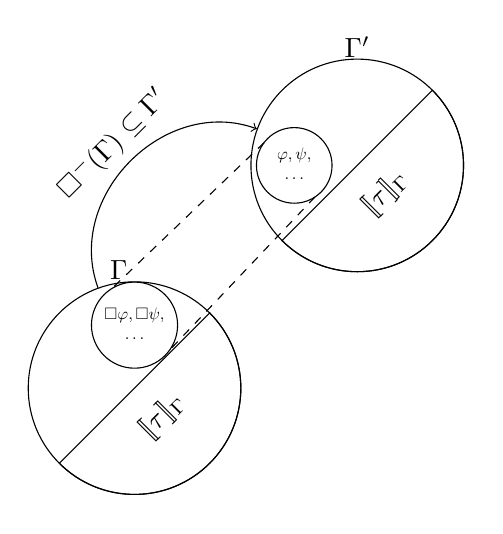
\begin{tikzpicture}[scale=2]
\pgfmathsetmacro{\felezesiszog}{45}
\pgfmathsetmacro{\sugar}{2.7}
\pgfmathsetmacro{\sugarv}{2.3}
\pgfmathsetmacro{\eltolas}{2}

\node[minimum size=\sugar cm, circle, draw=black](Gamma) at (0,0){};

\node[inner sep=0mm,draw,circle, minimum size=1.6cm,outer sep=0, scale=.6] (big) at ([shift=(90:4mm)]Gamma){$\begin{array}{c}\Box\varphi,\Box \psi,\\\dots \end{array}$};

\felkorvonal{\felezesiszog}{\sugar}
\begin{scope}[shift=(45:\eltolas cm)]
\felkorvonal{\felezesiszog}{\sugar}
\node[minimum size=\sugar cm, circle, draw=black](Gamma') at (0,0){};
\node[inner sep=0mm,draw,circle, minimum size=1.6cm,outer sep=0, scale=.6] (small)  at ([shift=(180:4mm)]Gamma'){$\begin{array}{c}\varphi,\psi,\\\dots \end{array}$};
%\node[yshift=7mm] at (small){$\Box^-(\Gamma)$};
\end{scope}

\draw[->] (Gamma) .. controls ([shift=(110:1.3cm)]Gamma) and ([shift=(160:1.3cm)]Gamma') .. node[midway, above, sloped]{$\Box^-(\Gamma) \subseteq \Gamma'$}(Gamma');

\draw[dashed] (tangent cs:node=small,point={(big.south west)},solution=2) -- (tangent cs:node=big,point={(small.south west)});

\draw[dashed] (tangent cs:node=small,point={(big.north east)},solution=1) -- (tangent cs:node=big,point={(small.north east)},solution=2);

\node[xshift=-2mm, yshift=15mm] at (Gamma){$\Gamma$};
\node[yshift=15mm] at (Gamma'){$\Gamma'$};
%\node[rotate=45] at (.5,1){$\Box^-(\Gamma) \subseteq \Gamma'$};
\node[rotate=45, xshift=0mm, yshift=-5mm] at (Gamma){$[\![\tau]\!]_\Gamma$};
\node[rotate=45, xshift=0mm, yshift=-5mm] at (Gamma'){$[\![\tau]\!]_\Gamma$};
%\node[rotate=45,xshift=-6mm, yshift=2mm] at (Gamma){$\mathsf r}=c_{2n}$};

\end{tikzpicture}}

\felirat{1}{1}{1}{3.5}{-3}
{\begin{tabular}{c} Truth Lemma\\ \hline \\[-2ex]
$\mathfrak M_{\mathrm L}, v_{\mathrm L}, \mu_{\mathrm L}, \gamma_{\mathrm L}, \Gamma \models \varphi \iff \varphi^{\mu, \gamma} \in \Gamma$
\end{tabular}}

\end{frame}


%\szakasz[Canonical Clock Models]{Canonical Clock Models}

\begin{frame}
	\frametitle{Canonical Collection of Clock Models}
\footnotesize
Now we will show that $\mathfrak C_{\mathrm L}$ is indeed a collection of clock model structures. Let

\[\overline{R}_{\mathrm{L}}\defegy \textup{the smallest equivalence relation containing $R_{\mathrm{L}}$.}\]

\bigskip

We will show that
\begin{center}\kemph{the $\overline R_{\mathrm L}$-connected parts of $\mathfrak C_{\mathrm L}$ can be considered as a clock model structure}.\end{center}

\bigskip

To refer to these models we will use the contained worlds as names \\ \hfill (like to refer to equivalence classes we use representatives).

\end{frame}



\begin{frame}[t]
	\frametitle{Canonical clock model structures}
\footnotesize

The canonical clock model structure of a canonical world $\Gamma$ will be

\[ \mathcal S_\mathrm{L}^\Gamma \defegy \left( W_{\mathrm{L}}^\Gamma, R_{\mathrm{L}}^\Gamma, Prop_{\mathrm{L}}^\Gamma, U_{{\mathrm L}}^\Gamma, \varnothing, \mathbb C_{\mathrm{L}}^\Gamma \right) \]
where
\begin{itemize}
\item $W_{\mathrm{L}}^\Gamma \defegy \{ \Gamma' \in W_\mathrm{L} \, : \, \Gamma \overline R _{\mathrm{L}}\Gamma' \}$
\item $R_{\mathrm{L}}^\Gamma \defegy R_\mathrm{L}\upharpoonright W_{\mathrm{L}}^\Gamma $
\item $Prop_{\mathrm{L}}^\Gamma \defegy \{ X\cap W_{\mathrm{L}}^\Gamma \, :\, X\in Prop_\mathrm{L}\} $
\item $\mathbb C_{\mathrm{L}}^\Gamma \defegy \{\wintension{}{\mathsf c} \upharpoonright W_{\mathrm{L}}^\Gamma \, : \, \mathsf{c}\in CC\}$
\end{itemize}

\end{frame}

\begin{frame}[t]
	\frametitle{$\mathcal S_{\mathrm{L}}^\Gamma$ is a clock model structure:}
\footnotesize

\begin{itemize}\footnotesize
\item $W_\mathrm{L}^\Gamma \neq \varnothing$ since $\Gamma \in W_\mathrm{L}^\Gamma$.
\pause
\item $R_\mathrm{L}^\Gamma \subseteq  (W_\mathrm{L}^\Gamma)^2$ by definition.
\pause
\item $(W, R, Prop)$ is a general frame, since $Prop_{\mathrm{L}}^\Gamma$ is a Boolean subalgebra of $\wp (W_\mathrm{L})$ and is closed to $R_{\mathrm{L}}^\Gamma$ by definition, so it is closed to $[R_{\mathrm{L}}^\Gamma]$ as well.
\pause
\item $U_{\mathrm{L}}^\Gamma$ is not empty since the set of rigid constants is not empty.
\pause
\item $\varnothing \notin U_{\mathrm{L}}^\Gamma$ since all the elements of $U_{\mathrm{L}}^\Gamma$ are equivalence classes of rigid constants, so each of these class are not empty.
\pause
\item $\mathbb C_{\mathrm{L}}^\Gamma$ is a set of functions defined on $W_\mathrm{L}^\Gamma$ by definition, and the values of these functions are either $\varnothing$ (again, by def.) or elements of $U_{\mathrm{L}}^\Gamma$; the latter the only one which needs a detailed proof.
\end{itemize}

\end{frame}

\begin{frame}[t]
\footnotesize
	\frametitle{$\mathcal S_{\mathrm{L}}^\Gamma$ is a clock model structure:}

\underline{\textsc{Lemma:}} All $\Gamma'\in W_{\mathrm L}^\Gamma$ share the same domain $U_{\mathrm{L}}^{\Gamma'}=U_{\mathrm{L}}^{\Gamma}$
\\ $\qquad$ \textsc{Proof:} $W_{\mathrm L}^\Gamma$ is connected, i.e., every world of it can be reached in finitely many back or forth step on $R_{\mathrm L}^\Gamma$. So it is enough to show that if $\Gamma_1 R_{\mathrm L}^\Gamma \Gamma_2$, i.e., $\Box ^- (\Gamma_1)\subseteq \Gamma_2$, then $\wintension{\Gamma_1}{\tau} = \wintension{\Gamma_2}{\tau}$:
    \begin{itemize}
     \item[(e)] $\wintension{\Gamma_1}{\tau} \subseteq \wintension{\Gamma_2}{\tau}$: Since $\mathrm{NI}\in \Gamma_1$, for all $\tau'\in \wintension{\Gamma_1}{\tau}$ it is true that $\Box \tau=\tau'\in \Gamma_1$, so $\tau=\tau'\in \Box^-(\Gamma_1)\subseteq \Gamma_2$, therefore $\tau'\in \wintension{\Gamma_2}{\tau}$. \hfill $\dashv$
     \item[(c)] $\wintension{\Gamma_1}{\tau} \supseteq \wintension{\Gamma_2}{\tau}$: Suppose that there is a $\tau'\in \wintension{\Gamma_2}{\tau}$ s.t. $\tau'\notin \wintension{\Gamma_1}{\tau}$. The latter means that $\tau'\neq \tau\in \Gamma_1$. Then by $\mathrm{NNI}\in \Gamma_1$, $\Box \tau'\neq \tau\in \Gamma_1$, therefore $\tau'\neq \tau\in \Box^-(\Gamma_1)\subseteq \Gamma_2$, therefore $\tau'\in \wintension{\Gamma_2}{\tau}$ which contradicts to our assumption. \hfill $\dashv$
    \end{itemize}
\pause

\underline{\textsc{Corollary:}} For all $\Gamma'\in W_{\mathrm L}^\Gamma$, if $\wintension[M_{\mathrm{L}}]{\Gamma'}{\mathsf c}\neq \varnothing$, then $\wintension[M_{\mathrm{L}}]{\Gamma'}{\mathsf c}\in U_{\mathrm{L}}^{\Gamma'} =U_{\mathrm{L}}^{\Gamma}$.

\underline{\textsc{Corollary:}} $\Gamma \overline R_{\mathrm{L}}\Gamma' \Longrightarrow \mathcal S_{\mathrm{L}}^{\Gamma} = \mathcal S_{\mathrm{L}}^{\Gamma'}$.
\\ \textsc{Proof:} By the lemma above we have $U_{\mathrm{L}}^{\Gamma'}=U_{\mathrm{L}}^{\Gamma}$. $\Gamma \overline R_{\mathrm{L}}\Gamma'$ implies $W_{\mathrm{L}}^{\Gamma} = W_{\mathrm{L}}^{\Gamma'}$, and every remaining component of the model structure are defined as relativizations/restrictions by $W_{\mathrm{L}}^{\Gamma'}$.

\end{frame}


\begin{frame}[t]
	\frametitle{Canonical clock models, \bemph{(CMM)}}
\footnotesize

The canonical clock model of a canonical world $\Gamma$ will be

\[ \mathfrak M_\mathrm{L}^\Gamma \defegy \left( \mathcal S_{\mathrm{L}}^{\Gamma}, \wintension[M_{\mathrm{L}}^{\textup{$\Gamma$}}]{}{\;}\right) \]
where
\begin{itemize}
\item $\intension[M_{\mathrm{L}}^{\textup{$\Gamma$}}]{\mathsf r} \defegy  \wintension{\Gamma}{\mathsf r} \bemph{{}\in U_\mathrm{L}^\Gamma}$
\item $\wintension[M_{\mathrm{L}}^{\textup{$\Gamma$}}]{}{\mathsf c} \defegy \wintension[C_{\mathrm{L}}]{}{\mathsf c}\upharpoonright W_{\mathrm{L}}^\Gamma \bemph{{}\in \mathbb C_\mathrm{L}^\Gamma}$
%\item $\intension[M_{\mathrm{L}}^{\textup{$\Gamma$}}]{\tau} \intension[M_{\mathrm{L}}^{\textup{$\Gamma$}}]{+} \intension[M_{\mathrm{L}}^{\textup{$\Gamma$}}]{\tau'} \defegy[0] \wintension{\Gamma}{\tau+\tau'} \bemph{{}\in U_\mathrm{L}^\Gamma}$
\item $\wintension{\Gamma}{\tau} \intension[M_{\mathrm{L}}^{\textup{$\Gamma$}}]{+} \wintension{\Gamma}{\tau'} \defegy[0] \wintension{\Gamma}{\tau+\tau'} \bemph{{}\in U_\mathrm{L}^\Gamma}$
%\item $\intension[M_{\mathrm{L}}^{\textup{$\Gamma$}}]{\tau} \intension[M_{\mathrm{L}}^{\textup{$\Gamma$}}]{\cdot} \intension[M_{\mathrm{L}}^{\textup{$\Gamma$}}]{\tau'} \defegy[0] \wintension{\Gamma}{\tau+\tau'} \bemph{{}\in U_\mathrm{L}^\Gamma}$
\item $\wintension{\Gamma}{\tau} \intension[M_{\mathrm{L}}^{\textup{$\Gamma$}}]{\cdot} \wintension{\Gamma}{\tau'} \defegy[0] \wintension{\Gamma}{\tau\cdot\tau'} \bemph{{}\in U_\mathrm{L}^\Gamma}$
\item $\intension[M_{\mathrm{L}}^{\textup{$\Gamma$}}]{\leq} \defegy \{\langle \wintension{\Gamma}{\tau},\wintension{\Gamma}{\tau'}\rangle  \bemph{{}\in (U_\mathrm{L}^\Gamma)^2} \, : \, \tau\leq\tau'\in \Gamma\}$
%\item $v_{\mathrm{L}}^\Gamma(p)\defegy\canintension[L]p \cap W_{\mathrm{L}}^\Gamma$
\end{itemize}

The Truth Lemma will be true only with the so-called canonical valuation $v_{\mathrm{L}}^\Gamma$:
\[ \Gamma' \in v_{\mathrm{L}}^\Gamma(p)\defekv p\in \Gamma', \quad \textup{ i.e., }\quad v_{\mathrm{L}}^\Gamma(p)\defekv \canintension[L]p \cap W_{\mathrm{L}}^\Gamma\]
Every substitution $\mu: NVar\to CMT$ gives a mathematical assignment on $\mathcal S_{\mathrm L}^\Gamma$:
\[\mu_{\mathrm{L}}^\Gamma (x) \defegy \wintension{\Gamma}{\mu (x)}\]
Every substitution $\gamma: CVar\to CC$ gives a clock assignment on $\mathcal S_{\mathrm L}^\Gamma$:
\[\gamma_{\mathrm{L}}^\Gamma (a)(\Sigma)\defegy \wintension{\Sigma}{\gamma (a)} \quad \textup{ where }\Sigma \in W_{\mathrm{L}}^\Gamma\]

\felirat{1}{1}{.9}{3.5}{0.5}{$\begin{array}{c}
        \textup{\underline{Truth Lemma}}
\\[1ex] \mathfrak M_{\mathrm L}^\Gamma, v_{\mathrm L}^\Gamma, \mu_{\mathrm L}^\Gamma, \gamma_{\mathrm L}^\Gamma, \Gamma \models \varphi
\\[1ex] \Updownarrow
\\[1ex] \varphi^{\mu, \gamma} \in \Gamma\end{array}$}

\end{frame}

\begin{frame}[t]
	\frametitle{Connected maximal sets name the same canonical model }
\footnotesize

\vspace{-.7cm}
\[ \Gamma \overline R_{\mathrm{L}}\Gamma' \Longrightarrow \mathfrak M_{\mathrm{L}}^{\Gamma} = \mathfrak M_{\mathrm{L}}^{\Gamma'}\]

\hrule

\bigskip

%$\mathcal S_{\mathrm{L}}^{\Gamma} = \mathcal S_{\mathrm{L}}^{\Gamma'}$, since
Suppose that $\Gamma \overline R_{\mathrm{L}}\Gamma'$. We showed before that $\mathcal S^\Gamma_\mathrm{L}= \mathcal S^{\Gamma'}_\mathrm{L}$.
\\ \bluebullet $  \wintension[M_{\mathrm{L}}^{\textup{$\Gamma$}}]{}{\mathsf c}
 = \wintension[C_{\mathrm{L}}]{}{\mathsf c}\upharpoonright W_{\mathrm{L}}^\Gamma
 = \wintension[C_{\mathrm{L}}]{}{\mathsf c}\upharpoonright W_{\mathrm{L}}^{\Gamma'}
 = \wintension[M_{\mathrm{L}}^{\textup{$\Gamma'$}}]{}{\mathsf c}$.
\\ \bluebullet For mathematical terms we have
$\wintension[M_{\mathrm{L}}^{\textup{$\Gamma$}}]{}{\tau}
 = \wintension{\Gamma}{\tau}
 \magyarazat{=}{\bemph{(e)},\bemph{(c)}} \wintension{\Gamma'}{\tau}
 = \wintension[M_{\mathrm{L}}^{\textup{$\Gamma'$}}]{}{\tau}$.
Finally, to show that $\wintension[M_{\mathrm{L}}^{\textup{$\Gamma$}}]{}{\leq} = \wintension[M_{\mathrm{L}}^{\textup{$\Gamma'$}}]{}{\leq}$, we use the observation that NO and NNO are canonical for this property:
    \begin{itemize}
     \item[($\mathrm{e_\leq}$)] $\wintension[M_{\mathrm{L}}^{\textup{$\Gamma$}}]{}{\leq} \subseteq \wintension[M_{\mathrm{L}}^{\textup{$\Gamma$}}]{}{\leq}$: By def. $\langle\wintension{\Gamma}{\tau},\wintension{\Gamma}{\tau'}\rangle \in \wintension[M_{\mathrm{L}}^{\textup{$\Gamma'$}}]{}{\leq}$ iff $\tau\leq \tau'\in \Gamma$.
         Since $\mathrm{NO}\in \Gamma$, by UG and UI we have that $\Box \tau\leq \tau'\in \Gamma$, so $\tau\leq \tau'\in \Box^-(\Gamma)\subseteq \Gamma'$, so by def. $\langle\wintension{\Gamma}{\tau},\wintension{\Gamma}{\tau'}\rangle \in \wintension[M_{\mathrm{L}}^{\textup{$\Gamma'$}}]{}{\leq}$. \hfill $\dashv$
     \item[($\mathrm{c_\leq}$)] $\wintension[M_{\mathrm{L}}^{\textup{$\Gamma$}}]{}{\leq} \supseteq \wintension[M_{\mathrm{L}}^{\textup{$\Gamma'$}}]{}{\leq}$:  Suppose that there is a $\langle\wintension{\Gamma}{\tau},\wintension{\Gamma}{\tau'}\rangle \in \wintension[M_{\mathrm{L}}^{\textup{$\Gamma'$}}]{}{\leq}$ s.t. $\langle\wintension{\Gamma}{\tau},\wintension{\Gamma}{\tau'}\rangle \notin \wintension[M_{\mathrm{L}}^{\textup{$\Gamma$}}]{}{\leq}$. The latter means that $\lnot\tau\leq \tau'\in \Gamma$. Then by $\mathrm{NNO}\in \Gamma$, $\Box \lnot \tau\leq \tau'\in \Gamma$, therefore $\lnot \tau'\leq \tau\in \Box^-(\Gamma)\subseteq \Gamma'$, therefore $\langle\wintension{\Gamma}{\tau},\wintension{\Gamma}{\tau'}\rangle \in \wintension[M_{\mathrm{L}}^{\textup{$\Gamma$}}]{}{\leq}$ which contradicts to our assumption. \hfill $\dashv$
    \end{itemize}

\end{frame}

\begin{frame}
	\frametitle{Corollary for Truth Lemma ($\Diamond$)}
\footnotesize


\underline{\textsc{Corollary:}} If $\Gamma \overline R_{\mathrm{L}}\Gamma'$,
\[ \mathfrak M_{\mathrm L}^{\Gamma}, v_{\mathrm L}^{\Gamma}, \mu_{\mathrm L}^{\Gamma}, \gamma_{\mathrm L}^{\Gamma}, \Sigma  \models \varphi
   \iff
   \mathfrak M_{\mathrm L}^{\kemph{\Gamma'}}, v_{\mathrm L}^{\kemph{\Gamma'}}, \mu_{\mathrm L}^{\kemph{\Gamma'}}, \gamma_{\mathrm L}^{\kemph{\Gamma'}}, \Sigma  \models \varphi\]
%since    $\mathfrak M_{\mathrm{L}}^{\Gamma} = \mathfrak M_{\mathrm{L}}^{\Gamma'}$ implies $W_{\mathrm{L}}^{\Gamma} = W_{\mathrm{L}}^{\Gamma'}$, and the functions $v_{\mathrm L}^{\Gamma'}, \mu_{\mathrm L}^{\Gamma'}, \gamma_{\mathrm L}^{\Gamma'}$ are defined as relativizations/restrictions by $W_{\mathrm{L}}^{\Gamma'}$
\end{frame}

\szakasz[Completeness]{Completeness}

\begin{frame}
\frametitle{Plan for strong completeness}
\footnotesize
%\[ \Gamma \derives[L^0] \varphi \quad \Leftarrow \quad \Gamma \models_{\mathrm{L}^0} \varphi \]
%\hrule
%\medskip

\begin{itemize}
\item Suppose indirectly that $\Gamma \not \derives[L^0]\varphi$.
\item Take a logic $\mathrm L$ which extends $\mathrm{L}^0$ with
\begin{itemize}
\item infinitely many new mathematical constants $MC^{\mathrm{new}}$, and
\item infinitely many new clock constants $CC^{\mathrm{new}}$.
\end{itemize}
So $MC^{\mathrm{new}}\cap MC_{\mathcal L^0}=\varnothing$ and $CC^{\mathrm{new}}\cap CC_{\mathcal L^0}=\varnothing$.
\\ $CMT^{\mathrm{new}} \defegy \bigcap \{ H\subseteq CMT_{\mathcal L} \, : \, MC^{\mathrm{new}}\subseteq H  \}$.
\item Take a set of constants
\begin{itemize}
\item $C_m\subseteq CMT^{\mathrm{new}}$, s.t. $C_m \geq \omega$, $CMT^{\mathrm{new}}-C_m\geq \omega$, and
\item $C_c\;\subseteq CC^{\mathrm{new}}$, \;\,\, s.t. $C_c \;\geq \omega$, \;\;\,\,$CC^{\mathrm{new}}-C_c\;\geq \omega$.
\end{itemize}
\item Take an arbitrary  $\mu:NVar \rightarrowtail C_m$  and $\gamma:CVar \rightarrowtail C_c$.
\item[CEL] %\bemph{\textsc{\underline{Conservative Extension Lemma:}}}
$\Gamma^{\mu, \gamma} \not \derives[L]\varphi^{\mu, \gamma}$.
\item $\Gamma^{\mu, \gamma} \cup\{\lnot\varphi^{\mu, \gamma}\}$ is $\mathrm{L}$-consistent.
\item[(I)]
%\bemph{\textsc{\underline{Inductivity Lemma:}}}
$\Gamma^{\mu, \gamma} \cup\{\lnot\varphi^{\mu, \gamma}\}$ is iTi in L.
\item[($\mathrm{L}^+$)] $\Gamma^{\mu, \gamma} \cup\{\lnot\varphi^{\mu, \gamma}\}$ is contained in a canonical world $\Gamma^+$
\item[(Truth)] $\mathfrak M_{\mathrm L}^\Gamma, v_{\mathrm L}^\Gamma, \mu_{\mathrm L}^\Gamma, \gamma_{\mathrm L}^\Gamma, \Gamma^+ \models \Gamma$ \quad but\quad  $\mathfrak M_{\mathrm L}^\Gamma, v_{\mathrm L}^\Gamma, \mu_{\mathrm L}^\Gamma, \gamma_{\mathrm L}^\Gamma, \Gamma^+ \not\models \varphi$
\item[(CMM)] Since the canonical model is a model indeed, $\Gamma \not\models \varphi$.
\end{itemize}
\end{frame}


\begin{frame}[t]
\frametitle{The use of \bemph{CEL}}
\footnotesize

Let $\mu:NVar \to C_m$ and $\gamma:CVar \to C_c $ be \cemph{injective}.

\[ \Gamma \not \derives[L^0]\varphi \mathrel{\Longrightarrow} \Gamma^{\mu, \gamma} \not \derives[L]\varphi^{\mu, \gamma}\]

\hrule
\bigskip

\[ \arraycolsep=.2mm
\begin{array}{rrclll}
   & \Gamma &\not \derives[L^0]& \varphi &\quad& \textup{assumption}
%\\ & \Gamma &\not \derives[L]& \varphi &\quad& \bemph{CEL}
\\ \forallin {\gamma_1, \dots , \gamma_n} \Gamma  & &\not \derives[L^0]& \gamma_1\lthen \cdots \gamma_n \lthen \varphi &\quad& \textup{synt.comp.}
\\ \forallin {\gamma_1, \dots , \gamma_n} \Gamma  & &\not \derives[L]& \gamma_1\lthen \cdots \gamma_n \lthen \varphi &\quad& \bemph{\mathrm{CEL}}: \textup{ Section 1.8}
\\ \forallin {\gamma_1, \dots , \gamma_n} \Gamma  & &\not \derives[L]& (\gamma_1\lthen \cdots \gamma_n \lthen \varphi)^{\;\mu, \gamma} &\quad& \textup{\cemph{GC${}^*$}:  Lemma~1.2.3.}
\\ \forallin {\gamma_1, \dots , \gamma_n} \Gamma  & &\not \derives[L]& \gamma_1^{\;\mu, \gamma}\lthen \cdots \gamma_n^{\;\mu, \gamma} \lthen \varphi^{\;\mu, \gamma} &\quad& \textup{}
\\ & \Gamma^{\;\mu, \gamma} &\not \derives[L]& \varphi^{\;\mu, \gamma} &\quad& \textup{q.e.d.}
\end{array}
\]

%\felirat{1}{1}{1}{3.6}{1.5}{
\[\mathrm{GC}^*\!\!: \quad \lrule{\varphi (\mathsf r_1/x_1, \dots , \mathsf r_k/x_k, \mathsf c_1/a_1, \dots, \mathsf c_n/a_n  )}{\varphi}
 \begin{array}{c} \textup{\cemph{if the constants are distinct}}\\\textup{and do not occur in $\varphi$}\end{array}\]

\bemph{Conservative Extension Lemma}:
\\$\mathcal L \defegy \mathcal L^0\cup C$ where $C$ is a set of new constants
\\ $\mathrm L\defegy$ the smallest set of $\mathcal L$ formulas that forms a logic including $\mathrm{L}^0$.

Then the logic $\mathrm{L}$ and $\mathrm{L}^0$ agree on $\mathrm L^0$-theorems, i.e.,
\[ \derives[L^0] \varphi \iff \derives[L]\varphi \qquad \textup{ for all }\varphi \in \mathcal L^0\]


\end{frame}

\begin{frame}[t]
\frametitle{\bemph{($\mathrm{I_m}$)}}
\scriptsize
%\begin{center}
$\Sigma $ is inductive in L, \\ \hfill if there is a set of mathematical constants $C'_m$ s.t. $C'_m\geq \omega$, and $C'_m\cap \mathrm{Const}(\Sigma)= \varnothing$.
%\end{center}
\smallskip

\hrule

\bigskip

\tiny
%\scalebox{.6}
{$\arraycolsep=.5mm \begin{array}{rclcl}
\Sigma &\derives[L]& \varphi(c/x) & \quad & \textup{for all $c\in CMT$; assumption}
\\                            &\derives[L]& \underbrace{\sigma_1\lthen \cdots \lthen \sigma_j\lthen \varphi(c/x)}_{\mathrm{Prf}} & \quad & \textup{assumption}
\\ && \textup{let }\{\mathsf r_1, \dots, \mathsf r_n\}= C'_m\cap \mathrm{Const(Prf)}-\{c\}, && C'_m\geq \omega
\\ && \textup{let }y_1, \dots, y_n, y\notin \mathrm{NVar(Prf)},
\\ && \textup{let }\mathbf s:= (y/c)(y_n/c_n)\cdots (y_1/c_1).
\\ &\derives[L]& (\sigma_1\lthen \cdots \lthen \sigma_j\lthen \varphi(c/x))\mathbf s&&  \mathrm{GC}
\\ &\derives[L]& (\sigma_1)\mathbf s\lthen \cdots \lthen (\sigma_j)\mathbf s\lthen (\varphi(c/x))\mathbf s
\\ &\derives[L]& \sigma_1\lthen \cdots \lthen \sigma_j\lthen (\varphi(c/x))\mathbf s &&  C'_m\cap \mathrm{Const}(\Sigma)= \varnothing
%\\ &\derives[L]& \forall \vec y\,[\sigma_1\lthen \cdots \lthen \sigma_j\lthen (\varphi(c/x))\mathbf s ]&& \mathrm{UG}
\\ &\derives[L]& \forall y_1\underbrace{\cdots \forall y_n\forall y[\sigma_1\lthen \cdots \lthen \sigma_j\lthen (\varphi(c/x))\mathbf s ]}_{F}&& \mathrm{UG}
\\[-1.5ex] &\derives[L]& \forall y_1 F \lthen F(c_1/y_1) && \mathrm{UI}
\\ &\derives[L]& \forall y_2\cdots \forall y_n\forall y[\sigma_1\lthen \cdots \lthen \sigma_j\lthen (\varphi(c/x))\mathbf s ](c_1/y_1)&& \mathrm{MP}
\\ &\vdots&&&\textup{eliminate the remained}
\\ &\derives[L]& \forall y[\sigma_1\lthen \cdots \lthen \sigma_j\lthen (\varphi(c/x))\mathbf s ](c_1/y_1)\cdots(c_n/y_n)&& \textup{indexed $\forall y_i$-s in the same way}
\\ &\derives[L]& \forall y[\sigma_1\lthen \cdots \lthen \sigma_j\lthen (\varphi(c/x))\mathbf s (c_1/y_1)\cdots(c_n/y_n)]&& \textup{$y_1, \dots ,y_n\notin \mathrm{Var}(\Sigma)$}
\\ &\derives[L]& \forall y[\sigma_1\lthen \cdots \lthen \sigma_j\lthen \varphi(c/x)(y/c)]&& \textup{$y_1, \dots ,y_n\notin \mathrm{Var}(\varphi)$}
\\ &\derives[L]& \forall y[\sigma_1\lthen \cdots \lthen \sigma_j\lthen \varphi(y/x)]&& c\notin \mathrm{Const}(\varphi)
\\ &\derives[L]& \sigma_1\lthen \cdots \lthen \sigma_j\lthen \forall y\varphi(y/x)&& y\notin \mathrm{Var}(\Sigma)
\\ &\derives[L]& \sigma_1\lthen \cdots \lthen \sigma_j\lthen \forall x\varphi&&
\\ \Sigma &\derives[L]& \forall x\varphi&& \textup{q.e.d.}
  \end{array}$}
\end{frame}

\begin{frame}[t]
\frametitle{\bemph{($\mathrm{I_c}$)}}
\scriptsize
$\Sigma $ is T-inductive in L, \\ \hfill if there is a set of clock constants $C'_c$ s.t. $C'_c\geq \omega$, $C'_c\cap \mathrm{Const}(\Sigma) = \varnothing$
\smallskip

\hrule

\bigskip

\normalsize

\scalebox{.6}{$\arraycolsep=.5mm \begin{array}{lrclcl}
   \forallin {\mathsf c}{CC}& \Sigma &\derives[L]& \BoxTemplate{\vec\varphi}\,(\mathcal E \mathsf c \lthen \psi (\mathsf c/a)) & \quad & \textup{assumption}
\\ \forallin {\mathsf c}{CC}& &\derives[L]& \sigma_1\lthen \cdots \lthen \sigma_n \lthen \BoxTemplate{\vec\varphi}\,(\mathcal E \mathsf c \lthen \psi (\mathsf c/a))
      & \quad & \textup{synt.comp.}
\\ \forallin {\mathsf c}{CC}&&\derives[L]& \BoxTemplate{\langle\sigma_1\land \cdots \land \sigma_n\land \varphi_1, \varphi_2, \dots, \varphi_n\rangle}\,(\mathcal E \mathsf c \lthen \psi (\mathsf c/a))
      & \quad & \textup{template lemma}
\\ &&\derives[L]& \BoxTemplate{\langle\sigma_1\land \cdots \land \sigma_n\land \varphi_1, \varphi_2, \dots, \varphi_n\rangle}\,(\mathcal E \mathsf c_i \lthen \psi (\mathsf c_i/a))
      && \textup{where $\mathsf c_i\in C'_c-\mathrm{Const}(\vec\varphi \cup \{\psi\})$}
\\ &&& && \textup{(there is such a $\mathsf c_i$ since $C'_c\geq \omega$)}
\\ &&\derives[L]& \kemph [\BoxTemplate{\langle\sigma_1\land \cdots \land \sigma_n\land \varphi_1, \varphi_2, \dots, \varphi_n\rangle}\,(\mathcal E \mathsf c_i \lthen \psi (\mathsf c_i/a))\kemph ](\mathsf c_j/a)
      && \textup{TI: $x\mapsto \mathsf c_j\in C'_c-(\mathrm{Const}(\vec\varphi \cup \{\psi\})\cup\{\mathsf c_i\})$}
\\& &\derives[L]& \kemph (\BoxTemplate{\langle\sigma_1\land \cdots \land \sigma_n\land \varphi_1, \varphi_2, \dots, \varphi_n\rangle(\mathsf c_j/a)\kemph )}\,(\mathcal E \mathsf c_i \lthen \psi (\mathsf c_i/a))
      && \textup{$x$ does not occur in$(\mathcal E \mathsf c_i \lthen \psi (\mathsf c_i/a))$}
\\& &\derives[L]& \BoxTemplate{\kemph (\langle\sigma_1\land \cdots \land \sigma_n\land \varphi_1, \varphi_2, \dots, \varphi_n\rangle(\mathsf c_j/a)\kemph )}\,(\mathcal E a \lthen \psi)
      && \textup{GC: $\mathsf c_i\mapsto a$}
\\& &\derives[L]& \BoxTemplate{\kemph (\langle\sigma_1\land \cdots \land \sigma_n\land \varphi_1, \varphi_2, \dots, \varphi_n\rangle(\mathsf c_j/a)\kemph )}\,\forall a \psi
      && \textup{\kemph{T$\forall$-Intro} ($a$ is not free in the template)}
\\& &\derives[L]& \kemph [\BoxTemplate{\langle\sigma_1\land \cdots \land \sigma_n\land \varphi_1, \varphi_2, \dots, \varphi_n\rangle }\,\forall a \psi \kemph](\mathsf c_j/a)
      && \textup{since $a$ is not free in $\forall a \psi$}
\\& &\derives[L]& \BoxTemplate{\langle\sigma_1\land \cdots \land \sigma_n\land \varphi_1, \varphi_2, \dots, \varphi_n\rangle}\,\forall a \psi
      && \textup{GC: $\mathsf c_j\mapsto a$}
\\& &\derives[L]& \sigma_1\lthen \cdots \lthen \sigma_n \lthen \BoxTemplate{\vec\varphi}\,\forall a \psi
      && \textup{template lemma}
\\& \Sigma&\derives[L]& \BoxTemplate{\vec\varphi}\,\forall a \psi
      && \textup{q.e.d.}
  \end{array}$}
\end{frame}




\begin{frame}[t]
\frametitle{The use of \bemph{(I)}}
\footnotesize

\begin{center}$\Gamma^{\mu, \gamma} \cup\{\lnot\varphi^{\mu, \gamma}\}$ is iTi in L. \end{center}

\hrule

\bigskip
%
%
% $C'_c := CC^{\mathrm{new}}-C_c$
% C'_c\cap \mathrm{Const}(\Gamma^{\mu, \gamma} \cup\{\lnot\varphi^{\mu, \gamma}\})= \varnothing
Since $\mu:NVar \rightarrowtail C_m$, we have that
\[\mathrm{MConst}(\Gamma^{\mu, \gamma} \cup\{\lnot\varphi^{\mu, \gamma}\}) \subseteq MC_{\mathcal L_0}\cup C_m \]
Let $C'_m := CMT^{\mathrm{new}}-C_m$.
\\ Since $C'_m\geq \omega$ and $C'_m\cap \mathrm{MConst}(\Gamma^{\mu, \gamma} \cup\{\lnot\varphi^{\mu, \gamma}\}) = \varnothing$ by the def. of $C_m$ and $\mu$,
\\ by $\bemph{(\mathrm{I_m})}$, $\Gamma^{\mu, \gamma} \cup\{\lnot\varphi^{\mu, \gamma}\}$ is inductive in L.

\bigskip

{\color{DeepSkyBlue3}\hrule}

\bigskip

Since $\gamma:CVar \rightarrowtail C_c$, we have that
\[\mathrm{CConst}(\Gamma^{\mu, \gamma} \cup\{\lnot\varphi^{\mu, \gamma}\}) \subseteq CC_{\mathcal L_0}\cup C_c \]
Let $C'_c := CC^{\mathrm{new}}-C_c$.
\\ Since $C'_c\geq \omega$ and $C'_c\cap \mathrm{CConst}(\Gamma^{\mu, \gamma} \cup\{\lnot\varphi^{\mu, \gamma}\}) = \varnothing$ by the def. of $C_c$ and $\gamma$,
\\ by $\bemph{(\mathrm{I_c})}$, $\Gamma^{\mu, \gamma} \cup\{\lnot\varphi^{\mu, \gamma}\}$ is T-inductive in L.

\end{frame}

\begin{frame}[t]
\frametitle{\bemph{($\mathrm{L}^+$)}}
\vspace{-1cm}

\begin{center} \scalebox{.7}{Every iTi $\mathrm{L}$-consistent set $\Sigma$ is extendable to an $\mathrm{L}$-maximal iTi $\Sigma^{+}$ one.}\end{center}

\smallskip

\hrule

\pause

\tiny

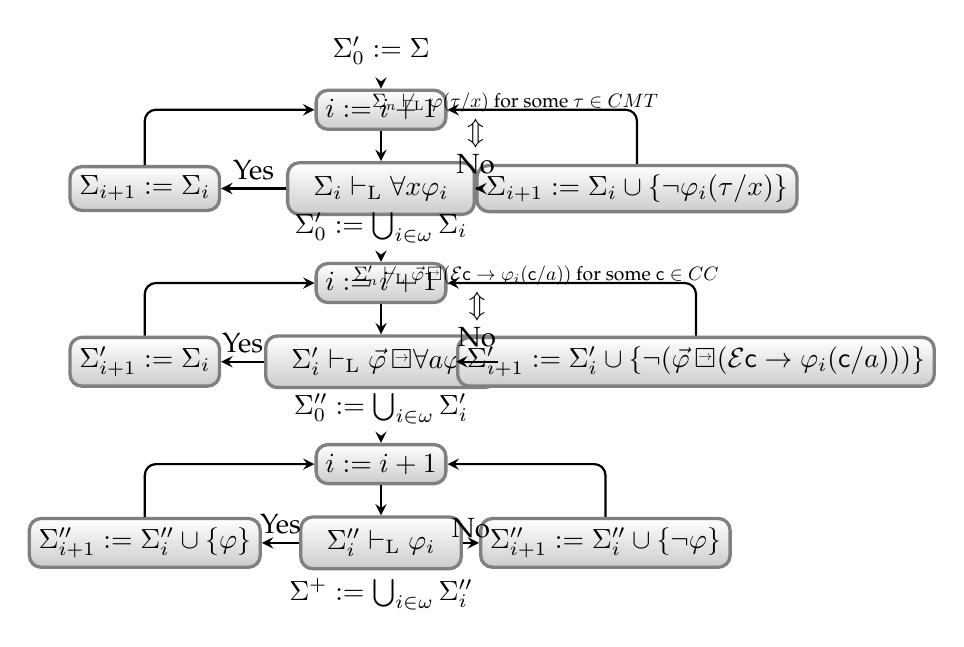
\begin{tikzpicture}[scale=1,>=stealth,
allapot/.style={ rectangle,rounded corners=1.5mm,very thick,draw=black!50,top color=white,bottom color=black!20,
}]

\pgfmathsetmacro{\magassag}{-1}
\node at (0,.75){$\Sigma'_0 := \Sigma$ };

\node(0) at (0,.45){};
\node[allapot](i) at (0,0){$i:=i+1$};

\node[allapot](test) at (0,\magassag){\begin{tabular}{c}
  $\Sigma_i \vdash_{\mathrm{L}} \forall x \varphi_i$
\end{tabular}};

\node[allapot](yes-case) at (-3,\magassag){$\Sigma_{i+1} := \Sigma_i%\cup \{\varphi_i(c/x_i)\}
$};
\node[allapot](no-case) at (3.25,\magassag){$\Sigma_{i+1} := \Sigma_i\cup \{ \lnot \varphi_i(\tau/x)\}$};

\begin{scope}[->, thick, rounded corners=4pt]
\draw (0)--(i);
\draw (i)--(test);
\draw (test)--(no-case) node[pos=.5, above, inner sep=.5mm]{\begin{tabular}{c} \hspace{1cm}\scalebox{.7}{$\Sigma_n \not \vdash_{\mathrm{L}} \varphi(\tau/x)$ for some $\tau\in CMT$} \\ $\Updownarrow$ \\ No \end{tabular}};
\draw (test)--(yes-case)node[pos=.5, above, inner sep=1mm]{Yes};
\draw (yes-case)|-(i);
\draw (no-case)|-(i);
\end{scope}


\node at (0,-1.5){$\Sigma'_0 := \bigcup_{i\in \omega} \Sigma_i$ };


\begin{scope}[yshift=-2.2cm]
\node(0) at (0,.45){};
\node[allapot](i) at (0,0){$i:=i+1$};

\node[allapot](test) at (0,\magassag){\begin{tabular}{c}
  $\Sigma_i' \vdash_{\mathrm{L}} \BoxTemplate {\vec \varphi}\forall a \varphi_i$
\end{tabular}};

\node[allapot](yes-case) at (-3,\magassag){$\Sigma'_{i+1} := \Sigma_i$};

\node[allapot](no-case) at (4,\magassag){$\Sigma'_{i+1} := \Sigma'_i\cup \{ \lnot (\BoxTemplate {\vec \varphi}\,(\mathcal E\mathsf c \to \varphi_i(\mathsf c/a)))\}$};

\begin{scope}[->, thick, rounded corners=4pt]
\draw (0)--(i);
\draw (i)--(test);
\draw (test)--(no-case) node[pos=.5, above, inner sep=.5mm]{\begin{tabular}{c} \hspace{1.5cm}\scalebox{.7}{$\Sigma_n' \not \vdash_{\mathrm{L}} \BoxTemplate {\vec \varphi}\,(\mathcal E\mathsf c \to \varphi_i(\mathsf c/a))$ for some $\mathsf c\in CC$} \\ $\Updownarrow$ \\ No \end{tabular}};
\draw (test)--(yes-case)node[pos=.5, above, inner sep=1mm]{Yes};
\draw (yes-case)|-(i);
\draw (no-case)|-(i);
\end{scope}
\end{scope}

\node at (0,-3.8){$\Sigma''_0 := \bigcup_{i\in \omega} \Sigma'_i$ };


\begin{scope}[yshift=-4.5cm]
\node(0) at (0,.45){};
\node[allapot](i) at (0,0){$i:=i+1$};

\node[allapot](test) at (0,\magassag){\begin{tabular}{c}
  $\Sigma_i'' \vdash_{\mathrm{L}} \varphi_i$
\end{tabular}};

\node[allapot](yes-case) at (-3,\magassag){$\Sigma''_{i+1} := \Sigma''_i\cup \{\varphi\}$};

\node[allapot](no-case) at (2.85,\magassag){$\Sigma''_{i+1} := \Sigma''_i\cup \{ \lnot \varphi\}$};

\begin{scope}[->, thick, rounded corners=4pt]
\draw (0)--(i);
\draw (i)--(test);
\draw (test)--(no-case) node[pos=.5, above, inner sep=.5mm]{No};
\draw (test)--(yes-case)node[pos=.5, above, inner sep=1mm]{Yes};
\draw (yes-case)|-(i);
\draw (no-case)|-(i);
\end{scope}
\end{scope}

\node at (0,-6.15){$\Sigma^+ := \bigcup_{i\in \omega} \Sigma''_i$ };

\end{tikzpicture}


{\scriptsize
\felirat{3}{1}{.7}{4.8}{2.25}{\textup{\begin{minipage}{3.6cm}
Suppose that $ \Sigma^+ \not \derives[L] \forall x \varphi$
\\ $\forallin \tau CMT \Sigma^+ \derives[L] \varphi (\tau/x).$
Then %the subset
$\Sigma_i\not \derives[L] \forall x \varphi$ either, so%, where $i$ is the step where $\forall \varphi_i= \forall x \varphi$.
%\\ So by the process,
\\ $\begin{tomb}[0.02]{rcl}\Sigma_{i+1}&=& \Sigma_{i}\cup\{\lnot \varphi (\tau/x)\} \\ &\subseteq& \Sigma^+\derives[L] \lnot \varphi (\tau/x). \end{tomb}$
\end{minipage}}}}


{\scriptsize
\felirat{3}{1}{.7}{4.6}{-3}{\textup{\begin{minipage}{4.4cm}
Suppose that \\ ${}\qquad \Sigma^+ \not \derives[L] \BoxTemplate{\vec \varphi}\forall a \varphi$
\\ but for all ${\mathsf c} \in CC$,
\\ $\Sigma^+ \derives[L] \BoxTemplate{\vec \varphi}( \mathcal E\mathsf c \lthen \varphi (\mathsf c/a)).$
\\ Then %the subset
$\Sigma_i\not \derives[L] \BoxTemplate{\vec \varphi}\forall a \varphi$ either, so
\\ $\begin{tomb}[0.02]{rcl}\Sigma_{i+1}&=& \Sigma_{i}\cup\{\lnot (\BoxTemplate{\vec \varphi}( \mathcal E\mathsf c \lthen \varphi (\mathsf c/a)))\} \\ &\subseteq& \Sigma^+\derives[L] \lnot (\BoxTemplate{\vec \varphi}( \mathcal E\mathsf c \lthen \varphi (\mathsf c/a))) \end{tomb}$
\end{minipage}}}}

\pause

\pecset{3}{\begin{tabular}{c}So $\Gamma^{\mu, \gamma} \cup\{\lnot\varphi^{\mu, \gamma}\}$ \\ is contained in a \\ canonical world $\Gamma^+$\end{tabular}}
\end{frame}

\szakasz[Truth Lemma]{Truth Lemma}

\begin{frame}
\frametitle{Truth Lemma}
\footnotesize
\begin{enumerate}\footnotesize
 \item \bemph{MALT}: Membership acts like truth
  \begin{itemize}\footnotesize
   \item Existence Lemma \bemph{(membership of $\Diamond \varphi$\dots)}
    \begin{itemize}\footnotesize
     \item \bemph{$(\Box^-)$}
     \item \bemph{(FE)}
    \end{itemize}
  \end{itemize}
 \item \bemph{SALA}: (Closed term) substitutions act like assignments
 \item Proof by induction on the complexity of formulas
\end{enumerate}
\end{frame}


\begin{frame}
\frametitle{\bemph{(MALT)} Membership acts like truth}
\footnotesize

If $\Gamma$ is $\mathrm{L}$-maximal, then  %\hfill  {\color{blue} $\Box^-(\Gamma) \defegy \{\varphi \, :\, \Box \varphi \in \Gamma\}$}
\[\begin{tomb}{rrcl}
   \bemph{\textup{consistent}} & \bot \notin \Gamma
%\\ \bemph{\textup{L-maximality}} & \top \in \Gamma
\\ \bemph{\textup{negation complete}} & \lnot \varphi \in \Gamma &\iff&\varphi \notin \Gamma
\\ \bemph{\textup{closed under $\derives[L]$}} & \varphi \land \psi \in \Gamma &\iff&\varphi \in \Gamma \textup{ and } \psi \in \Gamma
%\\ \bemph{\textup{L-maximality}} & \varphi \lor \psi \in \Gamma &\iff&\varphi \in \Gamma \textup{ or } \psi \in \Gamma
%\\ \bemph{\textup{L-maximality}} & \varphi \lthen \psi \in \Gamma &\iff&\varphi \in \Gamma \textup{ implies } \psi \in \Gamma
\\ \bemph{\textup{$R_{\mathrm{L}}$, ($\Box^-$), (FE), ($\mathrm{L}^+)$}} & \Diamond \varphi \in \Gamma &\iff &\existsp {\Gamma' \reflectbox{$R$}_{\mathrm{L}} \Gamma}\; \varphi \in \Gamma'
%\\ & \Box \varphi \in \Gamma &\iff &\forallp {\Gamma' \reflectbox{$R$}_{\mathrm{L}} \Gamma}\; \varphi \in \Gamma'
%\\ & \exists x \varphi \in \Gamma &\iff & \existsin {\tau} {D_{\mathrm L}(\Gamma)} \varphi (\tau/x)\in \Gamma
\\ \bemph{\textup{inductive, UI}}& \forall x \varphi \in \Gamma &\iff & \forallin {\tau}{CMT} \ \varphi(\tau/x)\in \Gamma
\\ \bemph{\textup{T-inductive, EI}}& \forall a \varphi \in \Gamma &\iff & \forallin {\mathsf c}{CC} \ \mathcal E\mathsf c \lthen \varphi(\mathsf c/a)\in \Gamma
\end{tomb}\]

The last case is the special case of T-inductivity, when the template is just $\varnothing$.

$\Diamond \Leftarrow$: Suppose that $\existsp {\Gamma' \supseteq \Box^-(\Gamma)}\ \varphi \in \Gamma'$ but
\[ \begin{tomb}[0.02]{rcl}
     \Diamond\varphi &\notin& \Gamma
\\   \lnot \Diamond\varphi &\in& \Gamma
\\   \Box \lnot \varphi &\in& \Gamma
\\   \lnot \varphi &\in& \Box^-(\Gamma)
\\   \lnot \varphi &\in& \Gamma'
\\   \bot &\in& \Gamma'
\end{tomb}\]
To the other direction we need the lemmas \bemph{($\Box^-$)}, \bemph{(FE)} and \bemph{($\mathrm{L}^+$)}.
\end{frame}

\begin{frame}
\frametitle{Existence Lemma}
\footnotesize
\begin{itemize}
 \item [\bemph{($\Box^-$)}] $\Box^- (\Gamma)$ inherits iTi from $\Gamma$.
 \item [\bemph{(FE)}]$\Box^- (\Gamma)\cup \{\varphi\}$ inherits iTi from $\Box^-(\Gamma)$.
 \item $\Box^-(\Gamma)\cup \{\varphi\}$ is consistent if $\Diamond \varphi \in \Gamma$, because if
\[ \begin{tomb}{rcl}
   \Box^- (\Gamma) \cup \{\varphi\}&\derives[L]&\bot
\\ \Box^- (\Gamma)&\derives[L]& \lnot \varphi
\\ \textup{\bemph{synt. compactness}}&\derives[L]& \chi_1 \lthen  \cdots \lthen \chi_{n}\lthen \lnot \varphi
\\ \textup{\bemph{RN + K-s }} &\derives[L]& \Box \chi_1 \lthen \cdots \lthen \Box\chi_{n}\lthen \Box \lnot \varphi
\\ \Box \chi_1, \cdots ,\Box\chi_{n} &\derives[L]& \Box \lnot \varphi
\\ \Gamma &\derives[L]& \Box \lnot \varphi
\\ \Gamma &\derives[L]& \lnot \Diamond\varphi
\\ \Gamma \cup \{ \Diamond \varphi \}&\derives[L]& \bot
\\ \Gamma &\derives[L]& \bot
\end{tomb}\]

 \item [\bemph{($\mathrm{L}^+$)}] There is a canonical world $\Gamma'$ extending $\Box^- (\Gamma)\cup \{\varphi\}$.
\end{itemize}
\end{frame}

\begin{frame}[t]
\frametitle{\bemph{($\Box^-$)}}
\footnotesize

If $\Gamma$ is inductive in $\mathrm{L}$, then so is $\Box^-(\Gamma)$:
\[ \arraycolsep=.2mm
\begin{array}{rclcl}
   \forallin {\tau}{CMT} \ \Box^- (\Gamma)&\derives[L]& \varphi (\tau/x)  &\quad& \textup{assumption}
\\ \forallin {\tau}{CMT} \ \Gamma &\derives[L]& \Box \varphi (c/x) && \textup{def. of. $\Box^-$}
\\ \Gamma &\derives[L]& \forall x \Box \varphi && \textup{$\Gamma$ is inductive in L}
\\ \Gamma &\derives[L]& \Box \forall x\varphi && \textup{BF}
\\ \Box^- (\Gamma)&\derives[L]& \forall x \varphi  && \textup{def.of $\Box^-$}
\end{array}
\]

If $\Gamma$ is T-inductive in $\mathrm{L}$, then so is $\Box^-(\Gamma)$:
\[ \arraycolsep=.2mm
\begin{array}{rclcl}
   \forallin {\mathsf c}{CC} \ \Box^- (\Gamma)&\derives[L]& \BoxTemplate{\vec \varphi}\,(\mathcal E \mathsf c \lthen \psi (\mathsf c/a)) &\quad& \textup{assumption}
\\ \forallin {\mathsf c}{CC} \ \Gamma &\derives[L]& \Box \BoxTemplate{\vec \varphi}\,(\mathcal E \mathsf c \lthen \psi (\mathsf c/a)) && \textup{def. of. $\Box^-$}
\\ \forallin {\mathsf c}{CC} \ \Gamma &\derives[L]& \BoxTemplate{\langle \top, \vec \varphi\rangle}\,(\mathcal E \mathsf c \lthen \psi (\mathsf c/a)) && \textup{template lemma}
\\ \Gamma &\derives[L]& \BoxTemplate{\langle \top, \vec \varphi\rangle}\forall a\psi  && \textup{$\Gamma$ is T-inductive in L}
\\ \Gamma &\derives[L]& \Box \BoxTemplate{\vec \varphi}\forall a\psi  && \textup{template lemma}
\\ \Box^- (\Gamma)&\derives[L]& \BoxTemplate{\vec \varphi}\forall a\psi  && \textup{def. of. $\Box^-$}
\end{array}
\]

\end{frame}

\begin{frame}[t]
\frametitle{\bemph{(FE)}}
\scriptsize
If $\Sigma$ is inductive then $\Sigma \cup \{\varphi\}$ is inductive as well.
\[\arraycolsep=.3mm \begin{array}{rrclcl}
   \forallin \tau {CMT}&\Sigma \cup \{\varphi\}&\derives[L]&\psi(\tau/x) &\qquad& \textup{assumption}
\\ \forallin \tau {CMT}&\Sigma &\derives[L]&\varphi \lthen \psi(\tau/x) && \textup{}
\\ \forallin \tau {CMT}&\Sigma &\derives[L]&[\varphi \lthen \psi(y/x)](\tau/y) && \textup{where $y$ does not occur in $\varphi$ and $\psi$}
\\                 &\Sigma &\derives[L]& \forall y[\varphi \lthen  \psi(y/x)] && \textup{inductivity of $\Sigma$}
\\                 &\Sigma &\derives[L]& \forall y\varphi \lthen  \forall y\psi(y/x) && \textup{UD}
\\                 &\Sigma &\derives[L]& \varphi \lthen \forall y \varphi && \textup{VQ}
\\                 &\Sigma &\derives[L]& \varphi \lthen  \forall y \psi(y/x) && \textup{chain rule}
\\                 &\Sigma &\derives[L]& \varphi \lthen  \forall x \psi &&
\\  &\Sigma \cup \{\varphi\}&\derives[L]&\forall x \psi && \textup{q.e.d.}
\end{array}\]

If $\Sigma$ is T-inductive then $\Sigma \cup \{\varphi\}$ is T-inductive as well.
\[\arraycolsep=.3mm \begin{array}{rrclcl}
   \forallin {\mathsf c} {CC} &\Sigma \cup \{\varphi\}&\derives[L]&\BoxTemplate{\vec\varphi}\,(\mathcal E\mathsf c \lthen \psi(\mathsf c/a)) &\quad& \textup{assumption}
\\ \forallin {\mathsf c} {CC} &\Sigma &\derives[L]&\varphi \lthen \BoxTemplate{\vec\varphi}\,(\mathcal E\mathsf c \lthen \psi(\mathsf c/a)) && \textup{ded.thm.}
\\ \forallin {\mathsf c} {CC} &\Sigma &\derives[L]&\BoxTemplate{\langle \varphi \land \varphi_1,\varphi_2, \dots , \varphi_n\rangle}\,(\mathcal E\mathsf c \lthen \psi(\mathsf c/a)) && \textup{template lemma}
\\ &\Sigma &\derives[L]&\BoxTemplate{\langle \varphi \land \varphi_1,\varphi_2, \dots , \varphi_n\rangle}\forall a \psi && \textup{$\Sigma$ is T-inductive}
\\ &\Sigma &\derives[L]&\varphi\lthen \BoxTemplate{\vec \varphi}\forall a \psi && \textup{template lemma}
\\ &\Sigma \cup \{\varphi\}&\derives[L]&\BoxTemplate{\vec \varphi}\forall a \psi && \textup{q.e.d.}
 \end{array}\]

\felirat{3}{1}{1}{4.35}{3}{$\Sigma = \Box^-(\Gamma)$}
\end{frame}


\begin{frame}[t]
\frametitle{\bemph{(SALA)} C.t. Substitutions act like assignments}
\scriptsize
$f$: and assignment $\mu: NVar\to CMT$ or $ \gamma: CVar \to CC$ and
\\ $v$: a variable from $NVar$ or $CVar$,
\\ $t$: a mathematical or clock term, respectively.
\[\begin{tomb}{rcl}
   \varphi^{\,f} &\defegy &\varphi \left(\,f(v_1)/v_1, \dots,\; f(v_{n})/v_{n}\right)
\\ \varphi^{\,f\setminus v_i} &\defegy &\varphi \left(\,f(v_1)/v_1, \dots, f(v_{i-i})/v_{i-i} , \kemph{v_i/v_{i}} ,f(v_{i+i})/v_{i+i} , \dots,\; f(v_{n})/v_{n}\right)
\\ \varphi^{\,f[t/v_i]} &\defegy &\varphi \left(\,f(v_1)/v_1, \dots, v_{i-i}/v_{i-i} , \kemph{t/v_{i}} , v_{i+i}/v_{i+i} , \dots,\; f(v_{n})/v_{n}\right)
\end{tomb}\]

\felirat{3}{1}{.7}{3}{2}{\begin{tabular}{l}
      $\varphi^{\mu}$ has no free mathematical variable
   \\ $\varphi^{\gamma}$ has no free clock variable
   \\ $\varphi^{\mu\setminus x_i}$ has at most $x_i$ free
   \\ ($\varphi^{\gamma\setminus a_i}$) has at most $a_i$ free
\end{tabular}}


Substitutions induce `almost-homomorphisms' on the terms and formulas:
\[\begin{tomb}{rcl}
   \mu(\tau +\tau') &\defegy &\mu(\tau) + \mu(\tau')
\\ \mu(\tau \cdot \tau') &\defegy &\mu(\tau) \cdot \mu(\tau')
\\ (P(t_1, \dots , t_n))^{\,f} &=& P(f(t_1), \dots, f(t_n))
\end{tomb}
\begin{tomb}{rcl}
   (\varphi \land \psi)^{\,f} &=& \varphi^{\,f} \land \psi^{\,f}
\\ (\lnot \varphi)^{\,f} &=& \lnot \varphi^{\,f}
\\ (\Box \varphi)^{\,f} &=& \Box \varphi^{\,f}
\\ (\forall v \varphi)^{\,f} &=& \forall v \varphi^{\,f\cemph{\setminus v}}
\end{tomb}\]

Closed term substitutions yield $f$-variations:
\[\begin{tomb}{rcl}
 (\varphi(t/v))^{\,f} &=& (\varphi(t/v))^{\,f\setminus v}
                          \magyarazat{=}{if $t$ is closed}  \varphi^{\,f\setminus v}(t/v)
                          =  \varphi^{\,f[t/ v]}
\end{tomb}
\]
\end{frame}

\begin{frame}[t]
\frametitle{\bemph{(SALA)} C.t. Substitutions act like assignments}
\scriptsize
If $\mu$ and $\gamma$ are closed term substitutions,
\[
   \wintension[M_{\mathrm{L}}^{\textup{$\Gamma$}}]{\mu_{\mathrm{L}}^\Gamma}{\tau}= \wintension{\Gamma}{\tau^{\mu}} \hspace{3cm}      \gamma_{\mathrm{L}}^\Gamma(a)(\Sigma)=\wintension{\Sigma}{a^\gamma}
\]
\hrule
\bigskip
\[\begin{tomb}{lllll}
   \mbox{\bluebullet}
     \wintension[M_{\mathrm{L}}^{\textup{$\Gamma$}}]{\mu_{\mathrm{L}}^\Gamma}{\mathsf r}
   = \wintension[M_{\mathrm{L}}^{\textup{$\Gamma$}}]{}{\mathsf r}
   = \wintension{\Gamma}{\mathsf r}
   = \wintension{\Gamma}{\mathsf r^{\mu}}
\\[1em] \mbox{\bluebullet}
     \wintension[M_{\mathrm{L}}^{\textup{$\Gamma$}}]{\mu_{\mathrm{L}}^\Gamma}{x}
   = \mu_{\mathrm{L}}^\Gamma(x)
   = \wintension{\Gamma}{\mu(x)}
   = \wintension{\Gamma}{x^{\mu}}
%\\[1em] \mbox{\bluebullet}
%     \wintension[M_{\mathrm{L}}^{\textup{$\Gamma$}}]{\mu_{\mathrm{L}}^\Gamma}{\tau + \tau'}
%   = \wintension[M_{\mathrm{L}}^{\textup{$\Gamma$}}]{\mu_{\mathrm{L}}^\Gamma}{\tau}
%     \wintension[M_{\mathrm{L}}^{\textup{$\Gamma$}}]{}{+}
%     \wintension[M_{\mathrm{L}}^{\textup{$\Gamma$}}]{\mu_{\mathrm{L}}^\Gamma}{\tau'}
%   = \wintension{\Gamma}{\tau^\mu}
%     \wintension[M_{\mathrm{L}}^{\textup{$\Gamma$}}]{}{+}
%     \wintension{\Gamma}{\tau'^\mu}
%   = \wintension{\Gamma}{\tau^\mu+\tau'^\mu}
%   = \wintension{\Gamma}{(\tau+\tau')^\mu}
\\[1em] \mbox{\bluebullet}
     \wintension[M_{\mathrm{L}}^{\textup{$\Gamma$}}]{\mu_{\mathrm{L}}^\Gamma}{\tau \cdot \tau'}
   = \wintension[M_{\mathrm{L}}^{\textup{$\Gamma$}}]{\mu_{\mathrm{L}}^\Gamma}{\tau}
     \wintension[M_{\mathrm{L}}^{\textup{$\Gamma$}}]{}{\cdot}
     \wintension[M_{\mathrm{L}}^{\textup{$\Gamma$}}]{\mu_{\mathrm{L}}^\Gamma}{\tau'}
   = \wintension{\Gamma}{\tau^\mu}
     \wintension[M_{\mathrm{L}}^{\textup{$\Gamma$}}]{}{\cdot}
     \wintension{\Gamma}{\tau'^\mu}
   = \wintension{\Gamma}{\tau^\mu\cdot\tau'^\mu}
   = \wintension{\Gamma}{(\tau\cdot\tau')^\mu}
\\[1em] \mbox{\bluebullet}
     \wintension[M_{\mathrm{L}}^{\textup{$\Gamma$}}]{\mu_{\mathrm{L}}^\Gamma}{\tau + \tau'} = \dots
%\\[1em] \mbox{\bluebullet}
%     \wintension[M_{\mathrm{L}}^{\textup{$\Gamma$}}]{\Sigma}{\mathsf c}
%   = \wintension{\Sigma}{\mathsf c}
%   = \left\{\begin{tomb}[0.1]{ll}
%             \textup{if } \mathsf c \ugyanaz \Sigma \tau \textup{ for some $\tau\in CMT$}:  &  \wintension{\Sigma}{\tau}
%          \\ \textup{if } \mathsf c \not\ugyanaz \Sigma \tau \textup{ for all $\tau\in CMT$}:& \varnothing
%            \end{tomb}\right.
\\[1em] \mbox{\bluebullet}
     \gamma_{\mathrm{L}}^\Gamma(a)(\Sigma)
%   = \gamma_{\mathrm{L}} (a)(\Sigma)
   = \wintension{\Sigma}{\gamma(a)}
   = \wintension{\Sigma}{a^\gamma}
%\\[1em] \tau
%   =\wintension[M_{\mathrm{L}}]{f}{\tau} \textup{ if $\tau$ is closed}
\end{tomb}\]

\felirat{3}{1}{.9}{3.5}{-4}{$\begin{tomb}{rcccl}
   \mu_{\mathrm{L}}^\Gamma (x) %&\defegy &\mu_{\mathrm{L}}(x)(\Gamma)
                                &\defegy& \wintension{\Gamma}{\mu(x)}
\\ \gamma_{\mathrm{L}}^\Gamma (a)(\Sigma)%&\defegy &\gamma_{\mathrm{L}} (a)(\Sigma)
                                          &\defegy& \wintension{\Sigma}{\gamma(a)}
\end{tomb}$}

\end{frame}

\begin{frame}[t]
\frametitle{\bemph{(SALA)} C.t. Substitutions act like assignments}
\scriptsize
If $\mu$ and $\gamma$ are closed term substitutions,
\[
   \mu_{\mathrm{L}}^\Gamma [x\mapsto \wintension{\Gamma}{\tau}]  = (\mu [\tau/x])_{\mathrm{L}}^\Gamma
 \hspace{3cm}
   \gamma_{\mathrm{L}}^\Gamma [a\mapsto \wintension{\Gamma}{\mathsf c}]  = (\gamma [\mathsf c/a])_{\mathrm{L}}^\Gamma
\]
\hrule
\bigskip
Let $y$ a variable that is different from $x$.
\[
\begin{tomb}[0.1]{rcl}
   \mu_{\mathrm{L}}^\Gamma [x\mapsto \wintension{\Gamma}{\tau}](x)
        &=& \wintension{\Gamma}{\tau}
\\[1ex] &=& \wintension{\Gamma}{\mu[\tau/x](x)}
\\[1ex] &=& (\mu[\tau/x])_{\mathrm{L}}^\Gamma (x)
\\[1ex]
\end{tomb}\qquad
\begin{tomb}[0.1]{rcl}
   \mu_{\mathrm{L}}^\Gamma [x\mapsto \wintension{\Gamma}{\tau}](y)
        &=& \mu_{\mathrm{L}}^\Gamma (y)
\\[1ex] &=& \wintension{\Gamma}{\mu(y)}
\\[1ex] &=& \wintension{\Gamma}{\mu[\tau/x](y)}
\\[1ex] &=& (\mu[\tau/x])_{\mathrm{L}}^\Gamma (y)
\end{tomb}\]
Let $b$ a variable that is different from $a$.
\[
\begin{tomb}[0.1]{rcl}
   \gamma_{\mathrm{L}}^\Gamma [a\mapsto \wintension{}{\mathsf c}]  (a)(\Sigma)
        &=& \wintension{\Sigma}{\mathsf c}
\\[1ex] &=& \wintension{\Sigma}{\gamma[\mathsf c/a](a)}
\\[1ex] &=& (\gamma[\mathsf c/a])_{\mathrm{L}}^\Gamma (a)(\Sigma)
\end{tomb}
\begin{tomb}[0.1]{rcl}
   \gamma_{\mathrm{L}}^\Gamma [a\mapsto \wintension{\Gamma}{\mathsf c}]  (b) (\Sigma)
        &=& \gamma_{\mathrm{L}}^\Gamma (b) (\Sigma)
\\[1ex] &=& \wintension{\Sigma}{\gamma(b)}
\\[1ex] &=& \wintension{\Sigma}{\gamma[\mathsf{c}/a](b)}
\\[1ex] &=& (\gamma[\mathsf{c}/a])_{\mathrm{L}}^\Gamma (b) (\Sigma)
\end{tomb}\]

\felirat{1}{1}{.9}{0}{-4.45}{$\begin{tomb}{rccclcrcccl}
   \mu_{\mathrm{L}}^\Gamma (x) %&\defegy &\mu_{\mathrm{L}}(x)(\Gamma)
                                &\defegy& \wintension{\Gamma}{\mu(x)}
&\qquad\qquad& \gamma_{\mathrm{L}}^\Gamma (a)(\Sigma) %&\defegy &\gamma_{\mathrm{L}} (a)(\Sigma)
                                                       &\defegy& \wintension{\Sigma}{\gamma(a)}
\end{tomb}$}

\end{frame}

\cimdia{Truth Lemma}

\begin{frame}[t]
\frametitle{Truth Lemma}\framesubtitle{propositional variables}
\scriptsize
\[
\mathfrak M_{\mathrm L}^\Gamma, v_{\mathrm L}^\Gamma, \mu_{\mathrm L}^\Gamma, \gamma_{\mathrm L}^\Gamma, \Gamma \models \varphi
\iff  \varphi^{\mu, \gamma} \in \Gamma\]
\hrule
\bigskip

\begin{itemize}
\item $\varphi \equiv p$ : propositional variables
 \[
  \begin{tomb}{rclll}
            \mathfrak M_{\mathrm L}^\Gamma, v_{\mathrm L}^\Gamma, \mu_{\mathrm L}^\Gamma, \gamma_{\mathrm L}^\Gamma, \Gamma  \models p
    &\iff & \Gamma \in v_{\mathrm L}^\Gamma(p)
     &\quad& \textup{def.of $\models$}
 \\[1ex]&\iff & p\in \Gamma
     &\quad& \textup{def.of $v_{\mathrm L}^\Gamma$}
 \\[1ex]&\iff & p^{\mu, \gamma}\in \Gamma
     &\quad& \textup{whatever}
 \end{tomb}\]
\end{itemize}
\end{frame}

\begin{frame}[t]
\frametitle{Truth Lemma}
\framesubtitle{Atomic mathematical formulas}
\scriptsize
\[
\mathfrak M_{\mathrm L}^\Gamma, v_{\mathrm L}^\Gamma, \mu_{\mathrm L}^\Gamma, \gamma_{\mathrm L}^\Gamma, \Gamma \models \varphi
\iff  \varphi^{\mu, \gamma} \in \Gamma\]
\hrule
\bigskip

\begin{itemize}
\item $\varphi \equiv \tau \leq \tau'$ : inequalities
 \[
  \begin{tomb}{rclll}
            \mathfrak M_{\mathrm L}^{\Gamma}, v_{\mathrm L}^\Gamma, \mu_{\mathrm L}^\Gamma, \gamma_{\mathrm L}^\Gamma, \Gamma  \models \tau\leq \tau'
    &\iff & \left\langle
             \wintension[\mathfrak M_{\mathrm L}^{\textup{$\Gamma$}}]{ \mu}{\tau},
             \wintension[\mathfrak M_{\mathrm L}^{\textup{$\Gamma$}}]{\mu}{\tau'}
            \right\rangle
            \in
            \wintension[\mathfrak M_{\mathrm L}^{\textup{$\Gamma$}}]{}{\leq}
     &\;& \textup{def.of $\models$}
\\[1ex] &\iff & \left\langle
             \wintension{\Gamma}{\tau^\mu},
             \wintension{\Gamma}{\tau'^\mu}
            \right\rangle
            \in
            \wintension[\mathfrak M_{\mathrm L}^{\textup{$\Gamma$}}]{}{\leq}
     && \textup{\bemph{(SALA)}}
\\[1ex] &\iff & \tau^\mu \leq \tau'^\mu \in \Gamma
     && \textup{def.of $\wintension[\mathfrak M_{\mathrm L}^{\textup{$\Gamma$}}]{}{\leq}$}
\\[1ex] &\iff & (\tau\leq \tau')^\mu \in \Gamma
     && \textup{}
\\[1ex] &\iff & (\tau\leq \tau')^{\mu, \gamma} \in \Gamma
     && \textup{}
 \end{tomb}\]
\item $\varphi \equiv \tau = \tau'$ : equalities
 \[
  \begin{tomb}{rclll}
            \mathfrak M_{\mathrm L}^{\Gamma}, v_{\mathrm L}^\Gamma, \mu_{\mathrm L}^\Gamma, \gamma_{\mathrm L}^\Gamma, \Gamma  \models \tau = \tau'
    &\iff & \wintension[\mathfrak M_{\mathrm L}^{\textup{$\Gamma$}}]{\mu}{\tau}= \wintension[\mathfrak M_{\mathrm L}^{\textup{$\Gamma$}}]{\mu}{\tau'}
     &\;& \textup{def.of $\models$}
\\[1ex] &\iff & \wintension{\Gamma}{\tau^\mu}= \wintension{\Gamma}{\tau'^\mu}
     && \textup{\bemph{(SALA)}}
\\[1ex] &\iff & \tau^\mu=\tau'^\mu\in \Gamma
     && \textup{def.of $\wintension{\Gamma}{\tau}$}
\\[1ex] &\iff & (\tau=\tau')^\mu\in \Gamma
     && \textup{}
\\[1ex] &\iff & (\tau=\tau')^{\mu, \gamma}\in \Gamma
     && \textup{}
 \end{tomb}\]
\end{itemize}
\end{frame}

\begin{frame}[t]
\frametitle{Truth Lemma}\framesubtitle{Atomic pointing formulas}
\scriptsize
\vspace{-3mm}
\[\mathfrak M_{\mathrm L}^\Gamma, v_{\mathrm L}^\Gamma, \mu_{\mathrm L}^\Gamma, \gamma_{\mathrm L}^\Gamma, \Gamma \models \varphi
\iff  \varphi^{\mu, \gamma} \in \Gamma\]
\hrule
\bigskip

\begin{itemize}
\item $\varphi \equiv \mathsf c :\tau$ : clock constant pointing
 \[
  \begin{tomb}{rclll}
            \mathfrak M_{\mathrm L}^{\Gamma}, v_{\mathrm L}^\Gamma, \mu_{\mathrm L}^\Gamma, \gamma_{\mathrm L}^\Gamma, \Gamma  \models \mathsf c :\tau
    &\iff &   \wintension[\mathfrak M_{\mathrm L}^{\textup{$\Gamma$}}]{}{\mathsf c}(\Gamma)
            = \wintension[\mathfrak M_{\mathrm L}^{\textup{$\Gamma$}}]{\mu}{\tau}
     &\;& \textup{def.of $\models$}
\\[1ex] &\iff &   \wintension{\Gamma}{\mathsf c}
            = \wintension{\Gamma}{\tau^\mu}
     &\;& \textup{def.of $\wintension[\mathfrak M_{\mathrm L}^{\textup{$\Gamma$}}]{}{\mathsf c}(\Gamma)$, \bemph{(SALA)}}
\\[1ex] &\iff &   (\exists \tau' : \mathsf c) \tau' = \tau^\mu\in \Gamma
     &\;& \textup{def.of $\wintension{\Gamma}{\mathsf c}$ and $\wintension{\Gamma}{\tau}$}
\\[1ex] &\iff &   \mathsf c:\tau^\mu\in \Gamma
     &\;& \textup{P$\!\triangle$}
\\[1ex] &\iff &   (\mathsf c :\tau)^{\mu}\in \Gamma
     &\;& \textup{}
\\[1ex] &\iff &   (\mathsf c :\tau)^{\mu, \gamma}\in \Gamma
     &\;& \textup{}
 \end{tomb}\]
\item $\varphi \equiv a :\tau$ : clock variable pointing
 \[
  \begin{tomb}{rclll}
            \mathfrak M_{\mathrm L}^{\Gamma}, v_{\mathrm L}^\Gamma, \mu_{\mathrm L}^\Gamma, \gamma_{\mathrm L}^\Gamma, \Gamma  \models a :\tau
    &\iff &   \gamma(a)(\Gamma)
            = \wintension[\mathfrak M_{\mathrm L}^{\textup{$\Gamma$}}]{\mu}{\tau}
     &\;& \textup{def.of $\models$}
\\[1ex] &\iff &   \wintension{\Gamma}{a^\gamma}
            = \wintension{\Gamma}{\tau^\mu}
     &\;& \textup{\bemph{(SALA)}}
\\[1ex] &\iff &   (\exists \tau' : a^\gamma) \tau' = \tau^\mu\in \Gamma
     &\;& \textup{def.of $\wintension{\Gamma}{a^\gamma}$ and $\wintension{\Gamma}{\tau}$}
\\[1ex] &\iff &   a^\gamma:\tau^\mu\in \Gamma
     &\;& \textup{P$\!\triangle$}
\\[1ex] &\iff &   (a :\tau)^{\mu, \gamma}\in \Gamma
     &\;& \textup{} \end{tomb}\]
\end{itemize}
\end{frame}

\begin{frame}[t]
\frametitle{Truth Lemma}\framesubtitle{Classical propositional connectives}
\scriptsize
\[
\mathfrak M_{\mathrm L}^\Gamma, v_{\mathrm L}^\Gamma, \mu_{\mathrm L}^\Gamma, \gamma_{\mathrm L}^\Gamma, \Gamma \models \varphi
\iff  \varphi^{\mu, \gamma} \in \Gamma\]
\hrule
\bigskip

\begin{itemize}
\item $\varphi \equiv \lnot \varphi$ : negation
 \[
  \begin{tomb}{rclll}
            \mathfrak M_{\mathrm L}^{\Gamma}, v_{\mathrm L}^\Gamma, \mu_{\mathrm L}^\Gamma, \gamma_{\mathrm L}^\Gamma, \Gamma  \models \lnot \varphi
    &\iff &   \mathfrak M_{\mathrm L}^{\Gamma}, v_{\mathrm L}^\Gamma, \mu_{\mathrm L}^\Gamma, \gamma_{\mathrm L}^\Gamma, \Gamma  \not \models \varphi
     &\;& \textup{def.of $\models$}
\\[1ex] &\iff & \varphi^{\mu, \gamma}\notin \Gamma
     &\;& \textup{ind.hip.}
\\[1ex] &\iff & \lnot \varphi^{\mu, \gamma}\in \Gamma
     &\;& \textup{neg. completeness}
\\[1ex] &\iff & (\lnot \varphi)^{\mu, \gamma}\in \Gamma
 \end{tomb}\]
\item $\varphi \equiv \varphi\land \psi$ : conjuction
 \[
  \begin{tomb}{rclll}
            \mathfrak M_{\mathrm L}^{\Gamma}, v_{\mathrm L}^\Gamma, \mu_{\mathrm L}^\Gamma, \gamma_{\mathrm L}^\Gamma, \Gamma  \models \varphi \land \psi
    &\iff &   \mathfrak M_{\mathrm L}^{\Gamma}, v_{\mathrm L}^\Gamma, \mu_{\mathrm L}^\Gamma, \gamma_{\mathrm L}^\Gamma, \Gamma  \models \varphi
              \textup{ and }
   \\[1ex]&&           \mathfrak M_{\mathrm L}^{\Gamma}, v_{\mathrm L}^\Gamma, \mu_{\mathrm L}^\Gamma, \gamma_{\mathrm L}^\Gamma, \Gamma  \models \psi     &\;& \textup{def.of $\models$}
\\[1ex]  &\iff & \varphi^{\mu, \gamma}\in \Gamma\textup{ and } \psi^{\mu, \gamma}\in \Gamma
     &\;& \textup{ind.hip.}
\\[1ex]  &\iff & \varphi^{\mu, \gamma}\land \psi^{\mu, \gamma}\in \Gamma
     &\;& \textup{deductively closed}
\\[1ex]  &\iff & (\varphi\land \psi)^{\mu, \gamma}\in \Gamma
 \end{tomb}\]
\end{itemize}
\end{frame}

\begin{frame}[t]
\frametitle{Truth Lemma}\framesubtitle{Modality}
\scriptsize
\[
\mathfrak M_{\mathrm L}^\Gamma, v_{\mathrm L}^\Gamma, \mu_{\mathrm L}^\Gamma, \gamma_{\mathrm L}^\Gamma, \Gamma \models \varphi
\iff  \varphi^{\mu, \gamma} \in \Gamma\]
\hrule
\bigskip

\begin{itemize}
\item $\varphi \equiv \Diamond \varphi$ : modality
 \[\hspace{-1cm}
  \begin{tomb}[.1]{rclll}
            \mathfrak M_{\mathrm L}^{\Gamma}, v_{\mathrm L}^\Gamma, \mu_{\mathrm L}^\Gamma, \gamma_{\mathrm L}^\Gamma, \Gamma  \models \Diamond \varphi
    &\iff & \existsp {\Gamma'\supseteq \Box^-(\Gamma)}  \; \mathfrak M_{\mathrm L}^{\Gamma}, v_{\mathrm L}^\Gamma, \mu_{\mathrm L}^\Gamma, \gamma_{\mathrm L}^\Gamma, \Gamma'  \models \varphi
     && \textup{def.of $\models$, $R_{\mathrm{L}}^{\Gamma}$}
\\[1ex] &\iff & \existsp {\Gamma'\supseteq \Box^-(\Gamma)} \; \mathfrak M_{\mathrm L}^{\Gamma'}, v_{\mathrm L}^{\Gamma'}, \mu_{\mathrm L}^{\Gamma'}, \gamma_{\mathrm L}^{\Gamma'}, \Gamma'  \models \varphi
     && \mathfrak M_{\mathrm{L}}^{\Gamma} = \mathfrak M_{\mathrm{L}}^{\Gamma'}
\\[1ex] &\iff & \existsp {\Gamma'\supseteq \Box^-(\Gamma)} \; \varphi^{\mu, \gamma}\in \Gamma'
     && \textup{ind.hip.}
\\[1ex] &\iff &  \Diamond\varphi^{\mu, \gamma}\in \Gamma'
     && \textup{Existence}
     \\ && &&\textup{Lemma,}
     \\ && &&\textup{\bemph{(MALT)}}
\\[1ex] &\iff &  (\Diamond\varphi)^{\mu, \gamma}\in \Gamma'
 \end{tomb}\]
\end{itemize}
\end{frame}

\begin{frame}[t]
\frametitle{Truth Lemma}\framesubtitle{Quantification}
\scriptsize
\[
\mathfrak M_{\mathrm L}^\Gamma, v_{\mathrm L}^\Gamma, \mu_{\mathrm L}^\Gamma, \gamma_{\mathrm L}^\Gamma, \Gamma \models \varphi
\iff  \varphi^{\mu, \gamma} \in \Gamma\]
\hrule
\bigskip

\begin{itemize}
\item $\varphi \equiv \forall x \varphi$ : mathematical quantification
 \[\hspace{-1.5cm}
  \begin{tomb}[.1]{rclll}
            \mathfrak M_{\mathrm L}^{\Gamma}, v_{\mathrm L}^\Gamma, \mu_{\mathrm L}^\Gamma, \gamma_{\mathrm L}^\Gamma, \Gamma  \models \forall x \varphi
    &\iff & \forallin {\wintension{L}{\tau}} {U_{\mathrm{L}}^\Gamma} \;\mathfrak M_{\mathrm L}^{\Gamma}, v_{\mathrm L}^\Gamma, \mu_{\mathrm L}^\Gamma [x\mapsto \wintension{L}{\tau}], \gamma_{\mathrm L}^\Gamma, \Gamma  \models \varphi
     && \textup{def.of $\models$, $U_{\mathrm{L}}^{\Gamma}$}
\\[1ex] &\iff & \forallin {\wintension{L}{\tau}} {U_{\mathrm{L}}^\Gamma} \;\mathfrak M_{\mathrm L}^{\Gamma}, v_{\mathrm L}^\Gamma, (\mu[\tau/x])_{\mathrm L}^\Gamma , \gamma_{\mathrm L}^\Gamma, \Gamma  \models \varphi
     && \textup{\bemph{(SALA)}}
\\[1ex] &\iff & \forallin {\tau} {CMT} \;\mathfrak M_{\mathrm L}^{\Gamma}, v_{\mathrm L}^\Gamma, (\mu[\tau/x])_{\mathrm L}^\Gamma , \gamma_{\mathrm L}^\Gamma, \Gamma  \models \varphi
     && \textup{}
\\[1ex] &\iff & \forallin {\tau} {CMT} \;\varphi^{\mu[\tau/x], \gamma} \in \Gamma
     && \textup{ind.hip.}
\\[1ex] &\iff & \forallin {\tau} {CMT} \;\varphi^{\mu\setminus x, \gamma}(\tau/x) \in \Gamma
     && \textup{\bemph{(SALA)}}
\\[1ex] &\iff & \forall x \varphi^{\mu\setminus x, \gamma} \in \Gamma
     && \textup{inductivity}
\\[1ex] &\iff & (\forall x \varphi)^{\mu, \gamma} \in \Gamma
     && \textup{the `almost'}
\\ && && \textup{part of hom.}
 \end{tomb}\]
\end{itemize}
\end{frame}

\begin{frame}[t]
\frametitle{Truth Lemma}\framesubtitle{Quantification}
\scriptsize
\[
\mathfrak M_{\mathrm L}^\Gamma, v_{\mathrm L}^\Gamma, \mu_{\mathrm L}^\Gamma, \gamma_{\mathrm L}^\Gamma, \Gamma \models \varphi
\iff  \varphi^{\mu, \gamma} \in \Gamma\]
\hrule
\bigskip

\begin{itemize}
\item $\varphi \equiv \forall a \varphi$ : clock quantification
\\[1em] $\hspace{-1.5cm}\mathfrak M_{\mathrm L}^{\Gamma}, v_{\mathrm L}^\Gamma, \mu_{\mathrm L}^\Gamma, \gamma_{\mathrm L}^\Gamma, \Gamma  \models \forall a \varphi \iff$
    \[
  \begin{tomb}[.1]{rclll}
   %         \mathfrak M_{\mathrm L}^{\Gamma}, v_{\mathrm L}^\Gamma, \mu_{\mathrm L}^\Gamma, \gamma_{\mathrm L}^\Gamma, \Gamma  \models \forall a \varphi
    &\iff & \forallin {\wintension{L}{\mathsf c}} {{\mathbb C_{\mathrm{L}}^\Gamma}_\Gamma} \;\mathfrak M_{\mathrm L}^{\Gamma}, v_{\mathrm L}^\Gamma, \mu_{\mathrm L}^\Gamma, \gamma_{\mathrm L}^\Gamma[a\mapsto \wintension{L}{\mathsf c}], \Gamma  \models \varphi
     && \textup{def.of $\models$, ${{\mathbb C_{\mathrm{L}}^\Gamma}_\Gamma}$}
\\[1ex] &\iff & \forallin {\wintension{L}{\mathsf c}} {{\mathbb C_{\mathrm{L}}^\Gamma}_\Gamma} \;\mathfrak M_{\mathrm L}^{\Gamma}, v_{\mathrm L}^\Gamma, \mu_{\mathrm L}^\Gamma , (\gamma[\mathsf c/a])_{\mathrm L}^\Gamma, \Gamma  \models \varphi
     && \textup{\bemph{(SALA)}}
\\[1ex] &\iff & \forallin {\mathsf c} {CC}(\existsin \tau {CMT} c:\tau \in \Gamma )\textup{ implies} \\ && \qquad \;\mathfrak M_{\mathrm L}^{\Gamma}, v_{\mathrm L}^\Gamma, \mu_{\mathrm L}^\Gamma , (\gamma[\mathsf c/a])_{\mathrm L}^\Gamma, \Gamma  \models \varphi
     && \textup{def.of ${{\mathbb C_{\mathrm{L}}^\Gamma}_\Gamma}$}
\\[1ex] &\iff & \forallin {\mathsf c} {CC}(\existsin \tau {CMT} c:\tau \in \Gamma )\Rightarrow\varphi^{\mu, \gamma[\mathsf c/a]} \in \Gamma
     && \textup{ind.hip.}
\\[1ex] &\iff & \forallin {\mathsf c} {CC}(\existsin \tau {CMT} c:\tau \in \Gamma )\Rightarrow\varphi^{\mu, \gamma\setminus a}(\mathsf c/a) \in \Gamma
     && \textup{\bemph{(SALA)}}
\\[1ex] &\iff & \forallin {\mathsf c} {CC} \exists x\,  c:x \in \Gamma \Rightarrow  \;\varphi^{\mu, \gamma\setminus a}(\mathsf c/a) \in \Gamma
     && \textup{UI}
\\[1ex] &\iff & \forallin {\mathsf c} {CC}\mathcal E \mathsf c \in \Gamma \Rightarrow \;\varphi^{\mu, \gamma\setminus a}(\mathsf c/a) \in \Gamma
     && \textup{def.of $\mathcal E(\mathsf c)$}
\\[1ex] &\iff & \forallin {\mathsf c} {CC}\mathcal E \mathsf c \lthen \varphi^{\mu, \gamma\setminus a}(\mathsf c/a) \in \Gamma
     && \textup{}
\\[1ex] &\iff & \forall a \varphi^{\mu, \gamma\setminus a} \in \Gamma
     && \textup{(T-)inductivity}
\\[1ex] &\iff & (\forall a \varphi)^{\mu, \gamma} \in \Gamma
     && \textup{the `almost'}
\\ && && \textup{part of hom.}
 \end{tomb}\]
\end{itemize}
\end{frame}

\begin{frame}
\frametitle{Conclusion}
\footnotesize
%Let L be any logic containing the axioms and closed to the rules we introduced on the slide Axiomatization, and the local semantic consequence relation $\models$ defined by models defined on the slide Clock models.

\underline{\textsc{Theorem:}} The smallest minimal clock logic is strongly complete w.r.t. the class of all clock models:
\[ \Gamma \derives[L] \varphi \mathrel{\Longleftarrow} \Gamma \models \varphi \]

\bigskip
\hrule
\bigskip

what is more, since our canonical models are all connected\dots

\bigskip

\underline{\textsc{Theorem:}}
The smallest minimal clock logic is strongly complete w.r.t. the class of all connected clock models:
\[ \Gamma \derives[L] \varphi \mathrel{\Longleftarrow} \Gamma \models^c \varphi \]
where
\begin{multline*}
\Gamma \models^c \varphi \defekv  \mathfrak M, v, \mu, \gamma, w \models \varphi \textup{ whenever } \mathfrak M, v, \mu, \gamma, w \models \Gamma \\ \textup{ for all connected $\mathfrak M$}\end{multline*}

\end{frame}

\end{document}
